
\documentclass{beamer}
\usecolortheme{dove}
\setbeamertemplate{navigation symbols}{}
\usepackage{amsmath,amssymb,amsfonts,amsthm, multicol, subfigure, color}
\usepackage{bm}
\usepackage{graphicx}
\usepackage{tabularx}
\usepackage{booktabs}
\usepackage{hyperref}
\usepackage{pdfpages}
\usepackage{xcolor}
\definecolor{seagreen}{RGB}{46, 139, 87}
\definecolor{mustard}{RGB}{234, 170, 0}
\def\independenT#1#2{\mathrel{\rlap{$#1#2$}\mkern2mu{#1#2}}}
\newcommand\indep{\protect\mathpalette{\protect\independenT}{\perp}}
\def\log{\text{log}}
\newcommand\logit{\text{logit}}
\newcommand\iid{\stackrel{\text{iid}}{\sim}}
\newcommand\E{\text{E}}
\newcommand\V{\text{V}}
\renewcommand\P{\text{P}}
\newcommand{\Cov}{\text{Cov}}
\newcommand{\Cor}{\text{Cor}}
\newcommand\doop{\texttt{do}}
\usepackage{stackrel}
\usepackage{tikz}
\usetikzlibrary{arrows,shapes.arrows,positioning,shapes,patterns,calc}
\newcommand\slideref[1]{\vskip .1cm \tiny \textcolor{gray}{{#1}}}
\newcommand\red[1]{\color{red}#1}
\newcommand\blue[1]{\color{blue}#1}
\newcommand\gray[1]{\color{gray}#1}
\newcommand\seagreen[1]{\color{seagreen}#1}
\newcommand\purple[1]{\color{purple}#1}
\newcommand\orange[1]{\color{orange}#1}
\newcommand\black[1]{\color{black}#1}
\newcommand\white[1]{\color{white}#1}
\newcommand\teal[1]{\color{teal}#1}
\newcommand\magenta[1]{\color{magenta}#1}
\newcommand\Fuchsia[1]{\color{Fuchsia}#1}
\newcommand\BlueGreen[1]{\color{BlueGreen}#1}
\newcommand\bblue[1]{\textcolor{blue}{\textbf{#1}}}
\newcommand\bred[1]{\textcolor{red}{\textbf{#1}}}
\newcommand\bgray[1]{\textcolor{gray}{\textbf{#1}}}
\newcommand\bgreen[1]{\textcolor{seagreen}{\textbf{#1}}}
\newcommand\bref[2]{\href{#1}{\color{blue}{#2}}}
\colorlet{lightgray}{gray!40}
\pgfdeclarelayer{bg}    % declare background layer for tikz
\pgfsetlayers{bg,main} % order layers for tikz
\newcommand\mycite[1]{\begin{scriptsize}\textcolor{darkgray}{(#1)}\end{scriptsize}}
\newcommand{\tcframe}{\frame{
%\small{
\only<1|handout:0>{\tableofcontents}
\only<2|handout:1>{\tableofcontents[currentsubsection]}}
%}
}

\newcommand{\goalsframe}{\begin{frame}{Learning goals for today}
By the end of class, you will be able to
\begin{itemize}
    \item conceptually trace the origins of racial wealth inequality to explicitly racist policies
    \item map racial segregation in a city of your choosing
\end{itemize} \vskip .2in
\end{frame}}

\usepackage[round]{natbib}
\bibliographystyle{humannat-mod}
\setbeamertemplate{enumerate items}[default]
\usepackage{mathtools}

\title{Studying Social Inequality with Data Science}
\author{Ian Lundberg}
\date{\today}

\begin{document}

\begin{frame}
\begin{tikzpicture}[x = \textwidth, y = \textheight]
\node at (0,0) {};
\node at (1,1) {};
\node[anchor = north west, align = left, font = \huge] at (0,.9) {Studying\\Social Inequality\\with Data Science};
\node[anchor = north east, align = right] (number) at (1,.9) {INFO 3370 / 5371\\Spring 2023};
\node[anchor = north, font = \Large, align = right] at (.5,.5) {\bblue{Political Origins of Wealth Inequality}};
\end{tikzpicture}
\end{frame}

\goalsframe

\begin{frame}
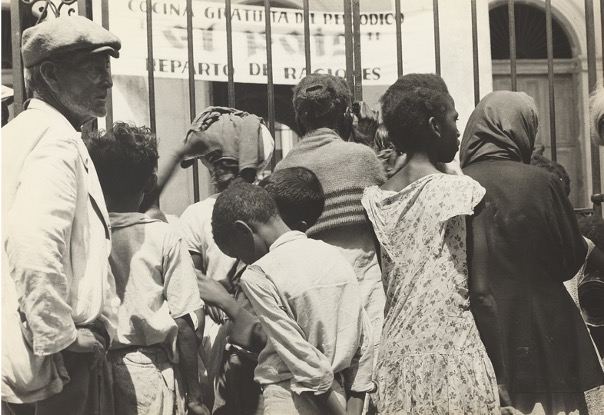
\includegraphics[height = .8\textheight]{figures/breadline}\\
\begin{footnotesize}
Walker Evans, 1933. The Breadline.\\
Source: \href{https://www.nga.gov/learn/teachers/lessons-activities/uncovering-america/great-depression.html}{National Gallery of Art}
\end{footnotesize}
\end{frame}

\begin{frame}
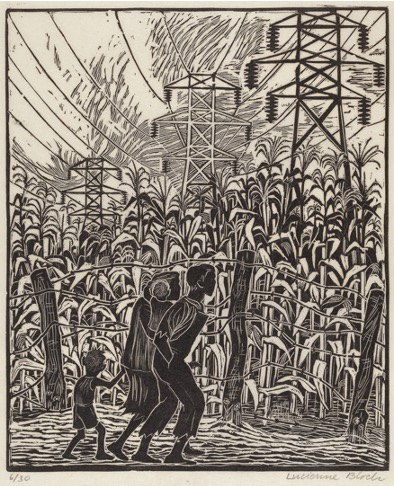
\includegraphics[height = .8\textheight]{figures/land_of_plenty}\\
\begin{footnotesize}
Lucienne Bloch, 1936. Land of Plenty.\\
Source: \href{https://www.nga.gov/learn/teachers/lessons-activities/uncovering-america/great-depression.html}{National Gallery of Art}
\end{footnotesize}
\end{frame}

\begin{frame}
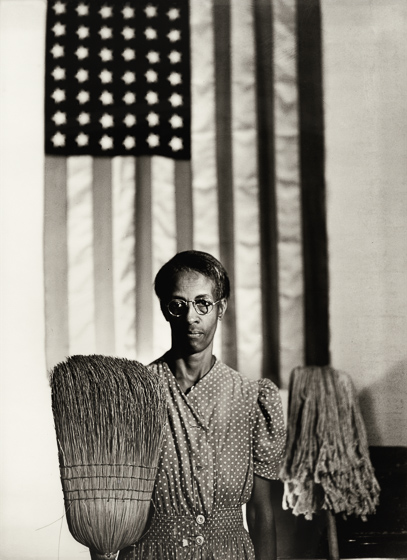
\includegraphics[height = .85\textheight]{figures/Parks-Charwoman-WSS}\\
\begin{footnotesize}
Gordon Parks, 1942. Washington, D.C. Government Charwoman (American Gothic).\\
Source: \href{https://www.nga.gov/learn/teachers/lessons-activities/uncovering-america/great-depression.html}{National Gallery of Art}
\end{footnotesize}
\end{frame}

\begin{frame}
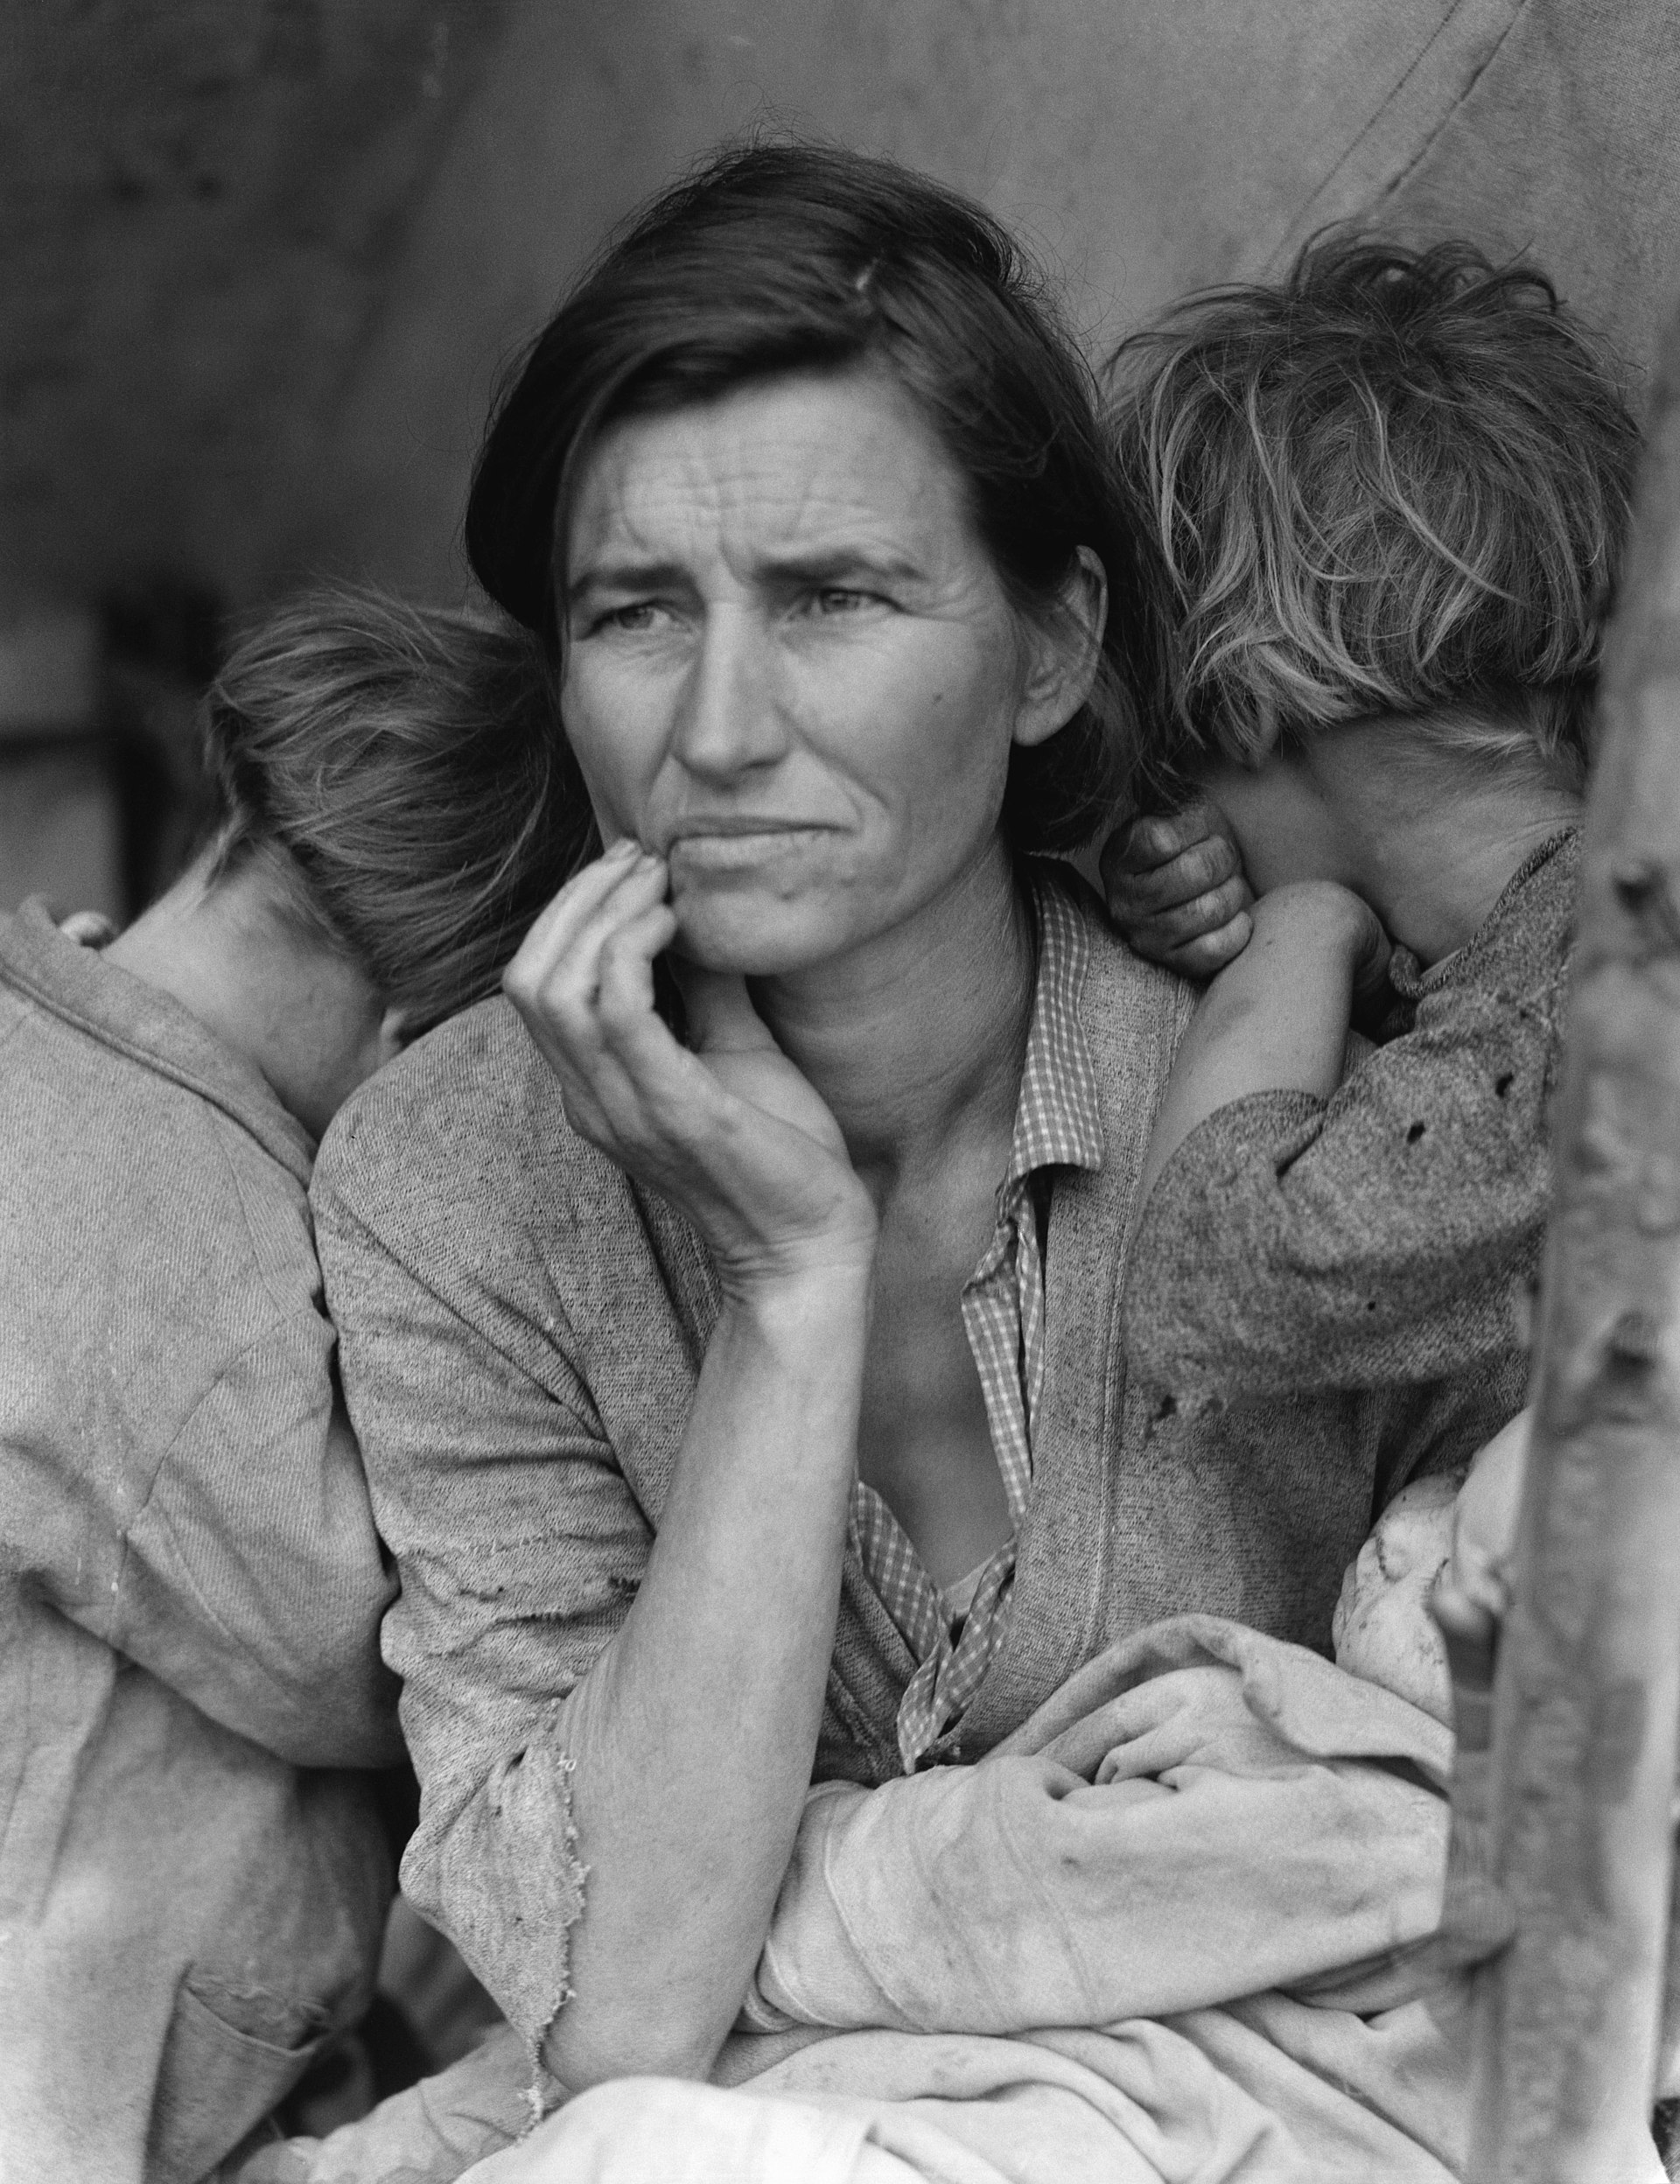
\includegraphics[height = .85\textheight]{figures/Lange-MigrantMother}\\
\begin{footnotesize}
Dorothea Lange, 1936. Migrant Mother.\\
Source: \href{https://en.wikipedia.org/wiki/Migrant_Mother}{Wikimedia}, original in MOMA NY
\end{footnotesize}
\end{frame}

\begin{frame}
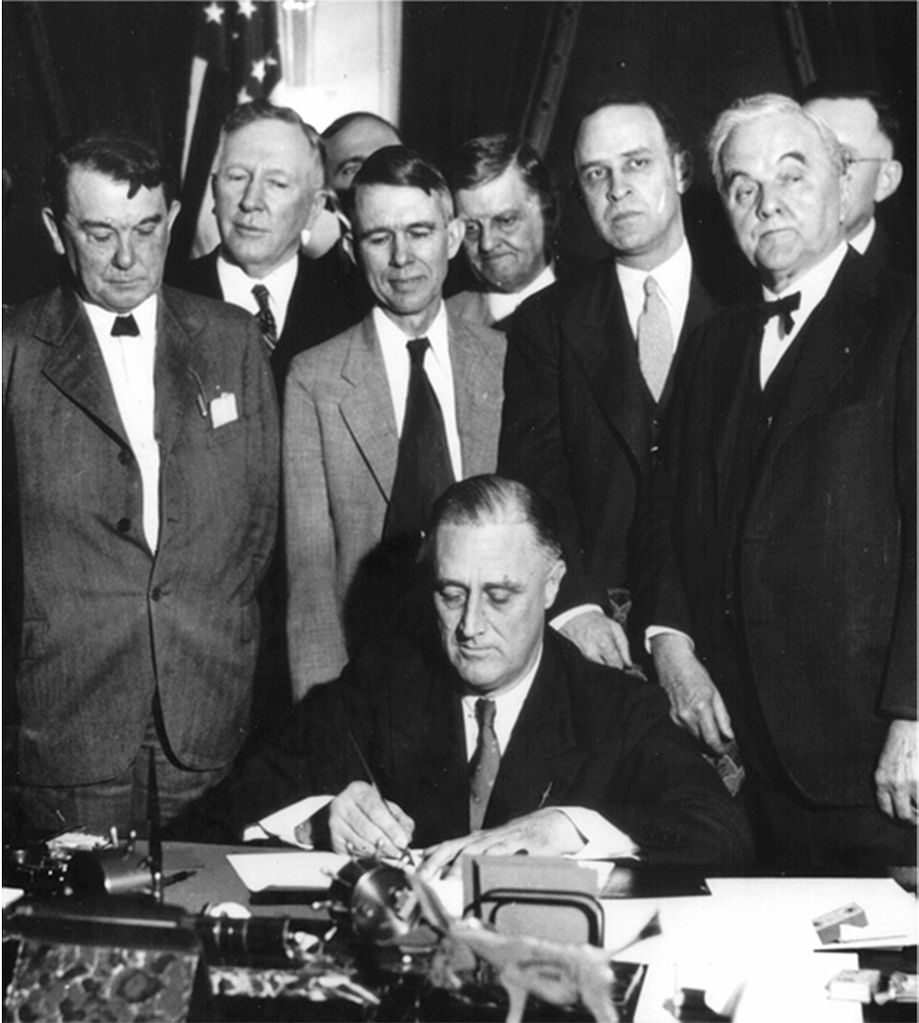
\includegraphics[width = .7\textwidth]{figures/fdr_tva}\\
Source: \href{https://commons.wikimedia.org/wiki/File:Roosevelt_signing_TVA_Act_(1933).jpg}{Wikimedia}
\end{frame}

\begin{frame}
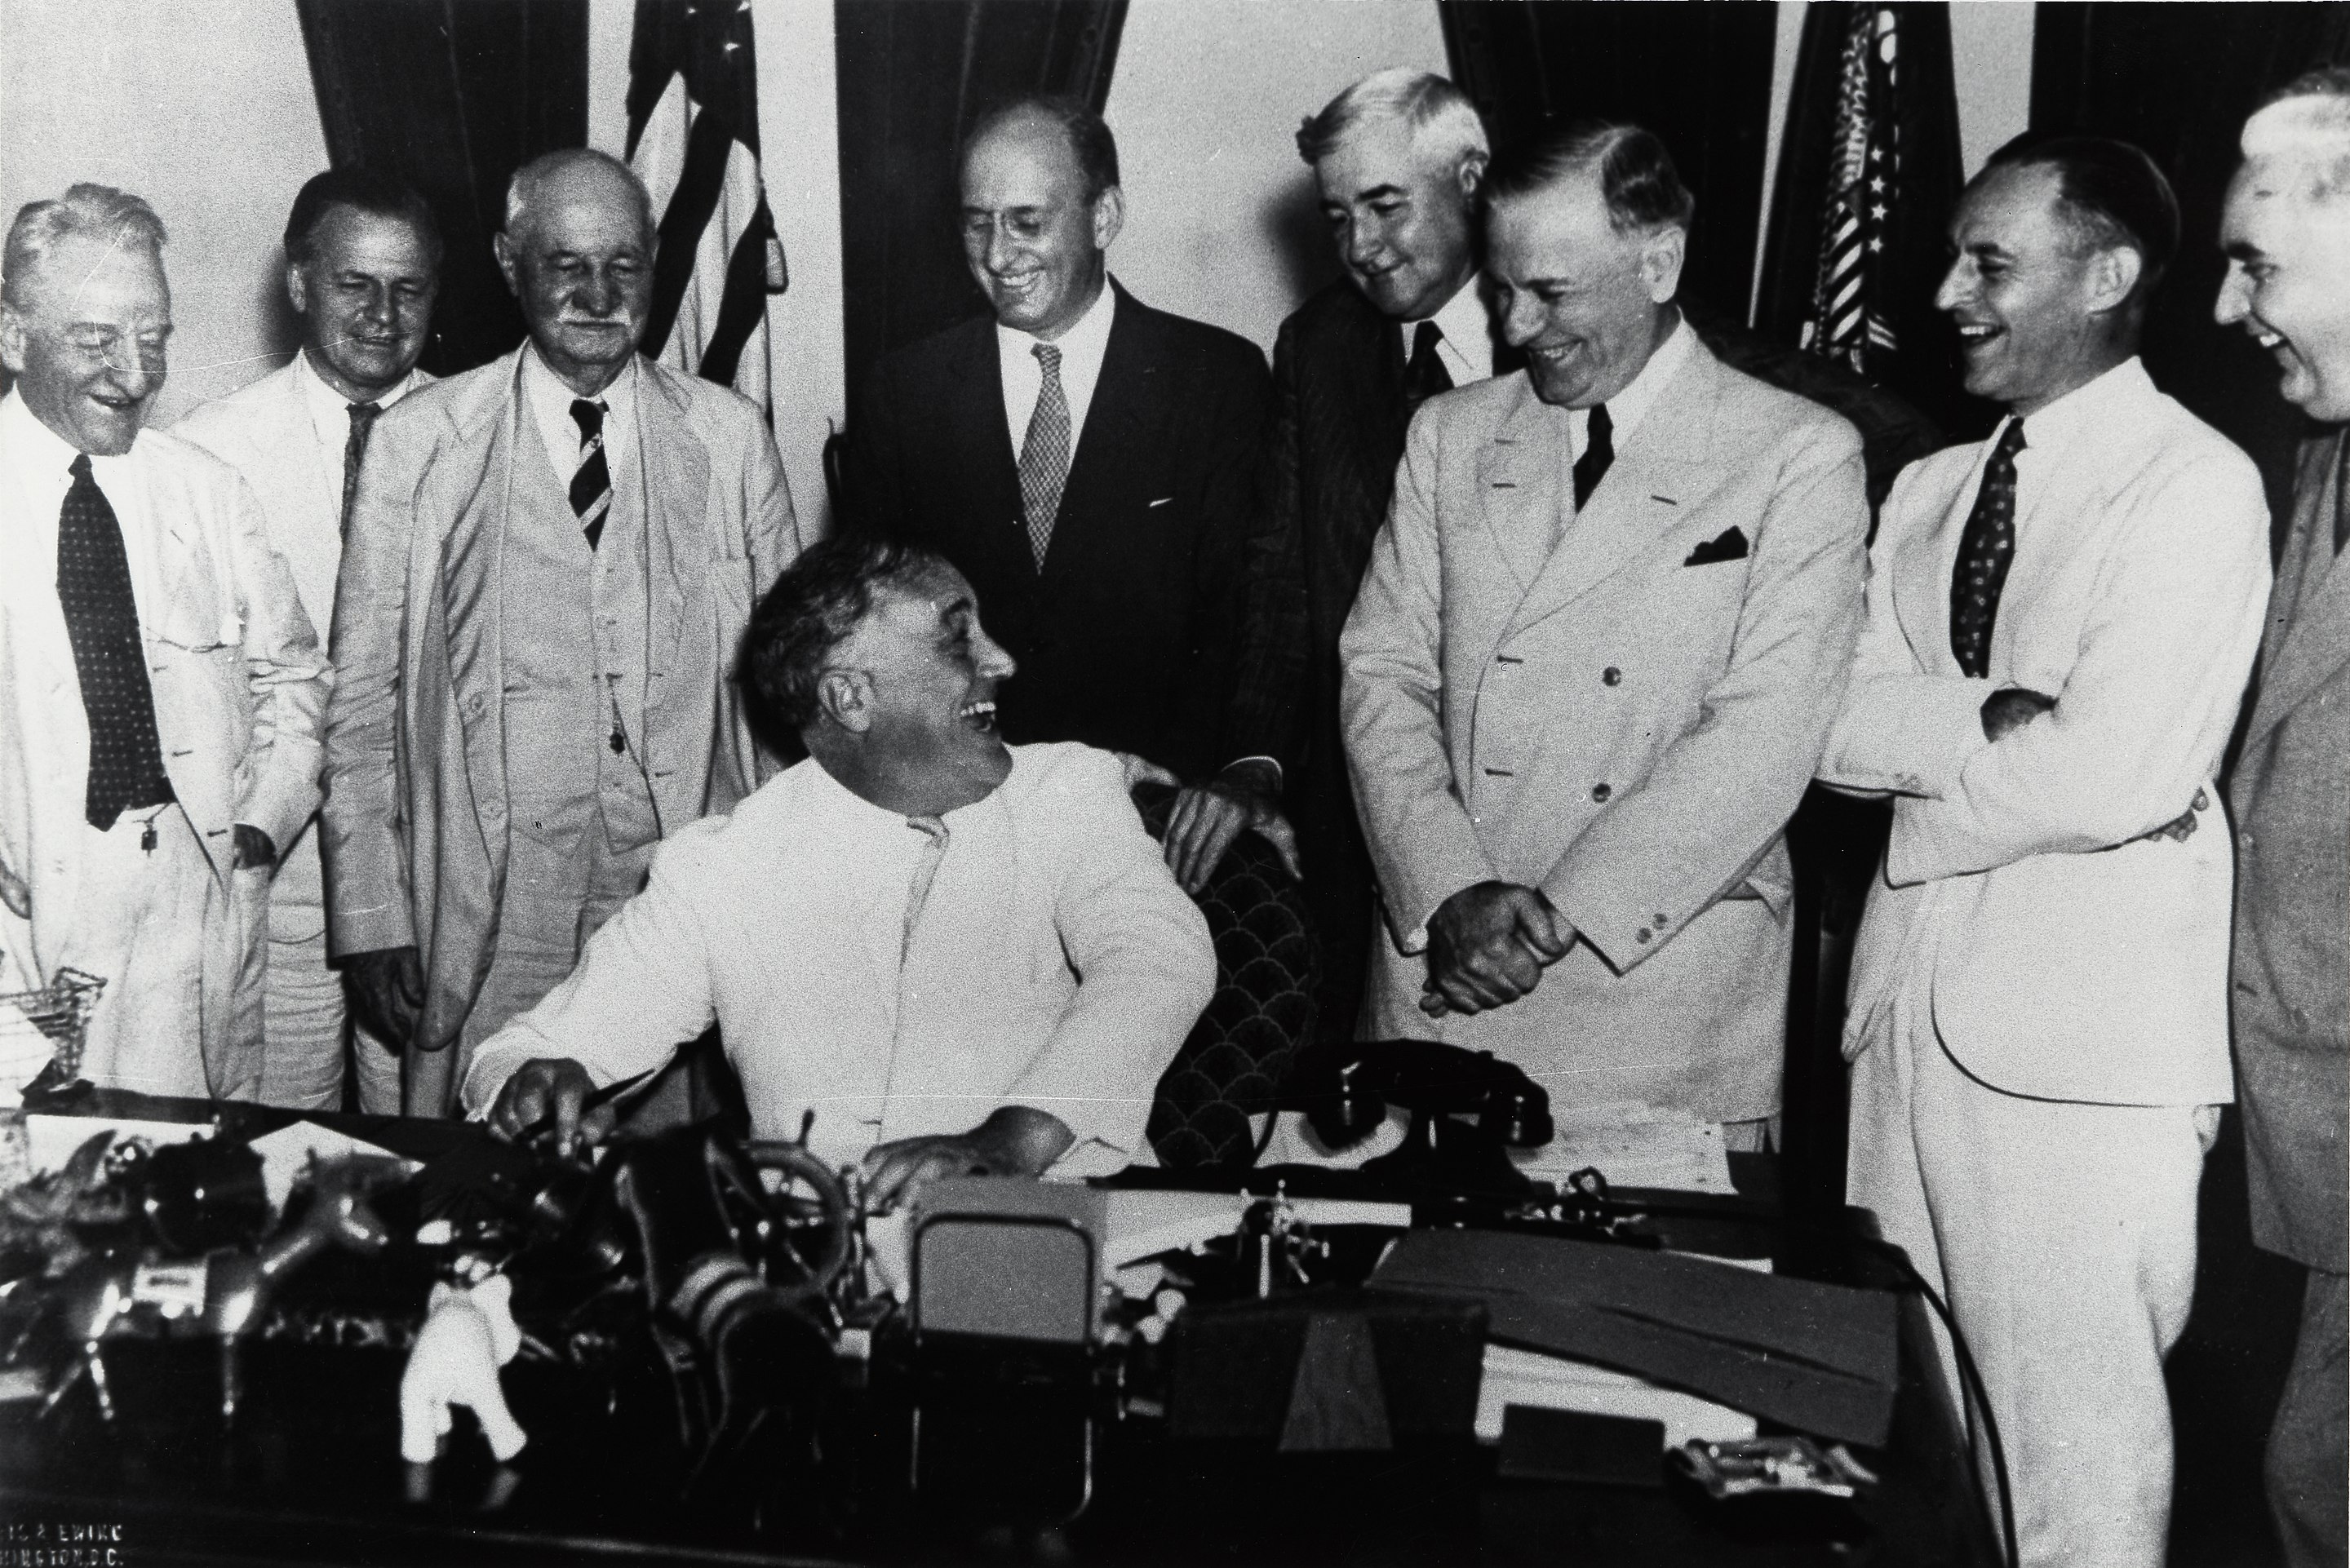
\includegraphics[width = .7\textwidth]{figures/fdr_banking}\\
Source: \href{https://commons.wikimedia.org/wiki/File:Franklin_Delano_Roosevelt_signs_Banking_Act_of_1935.jpg}{Wikimedia}
\end{frame}

\begin{frame}
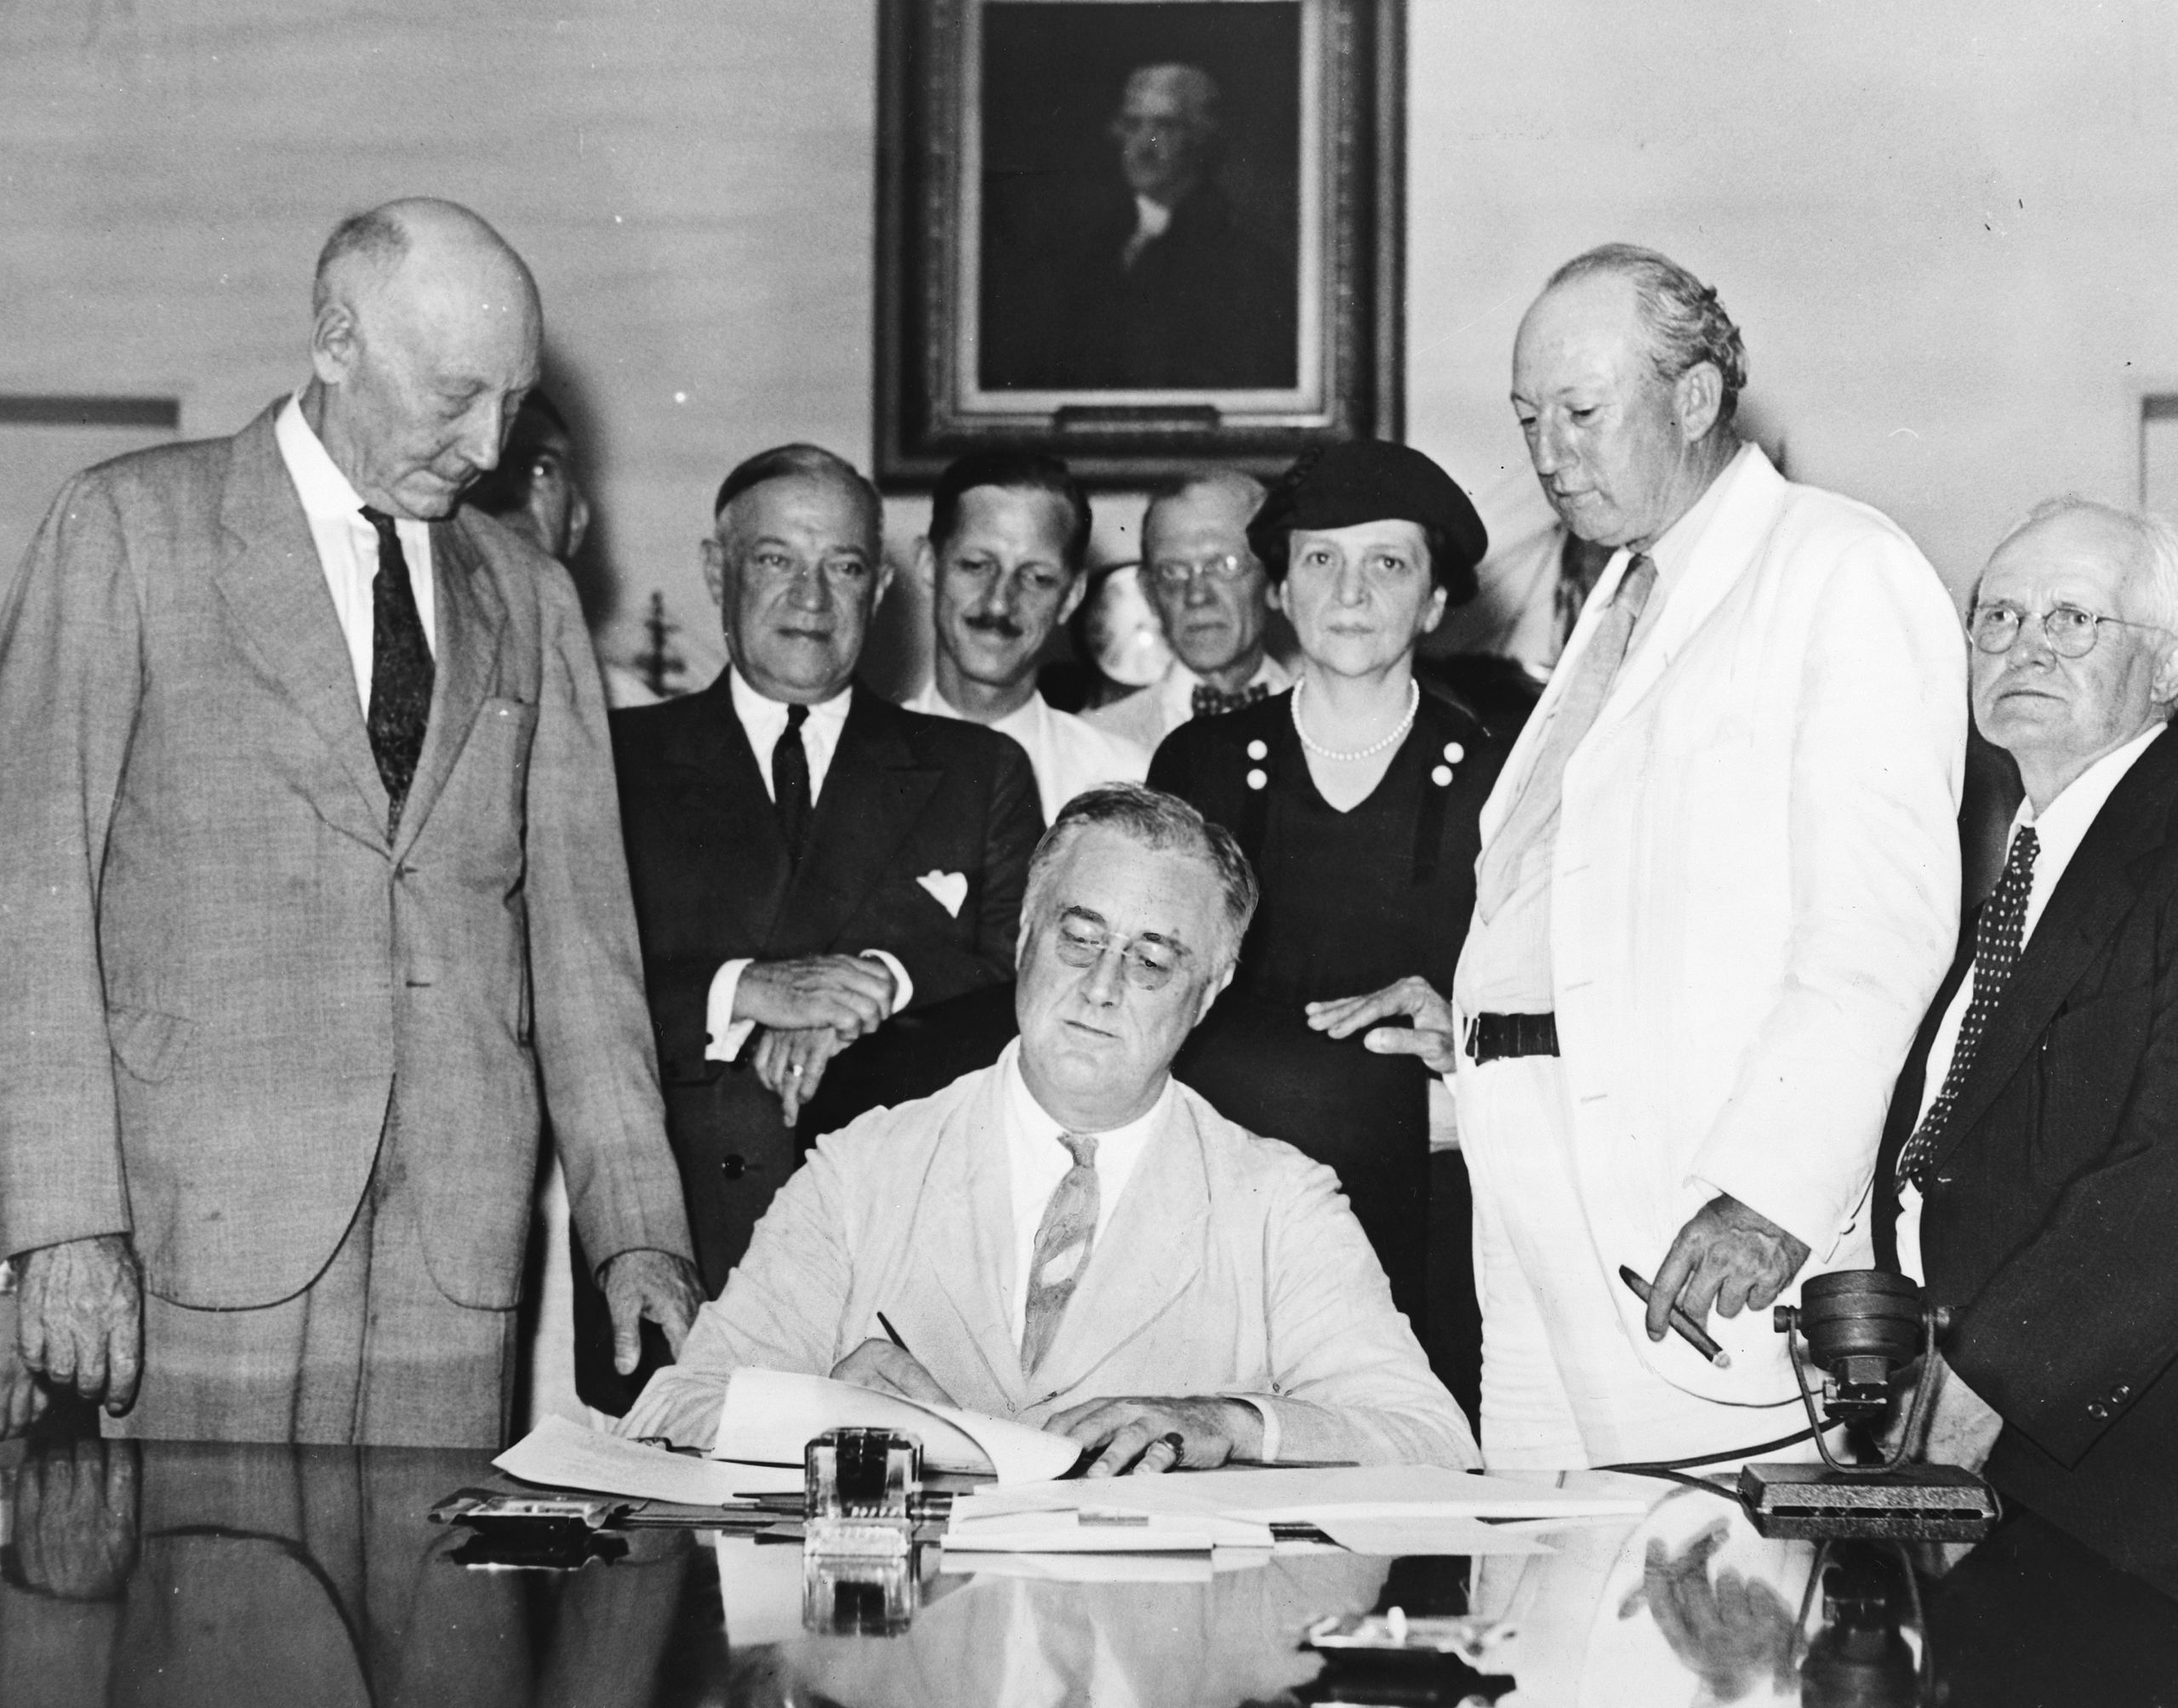
\includegraphics[width = .7\textwidth]{figures/fdr_ssa}\\
Source: \href{https://commons.wikimedia.org/wiki/File:Signing_Of_The_Social_Security_Act.jpg}{Wikimedia}
\end{frame}

\begin{frame}
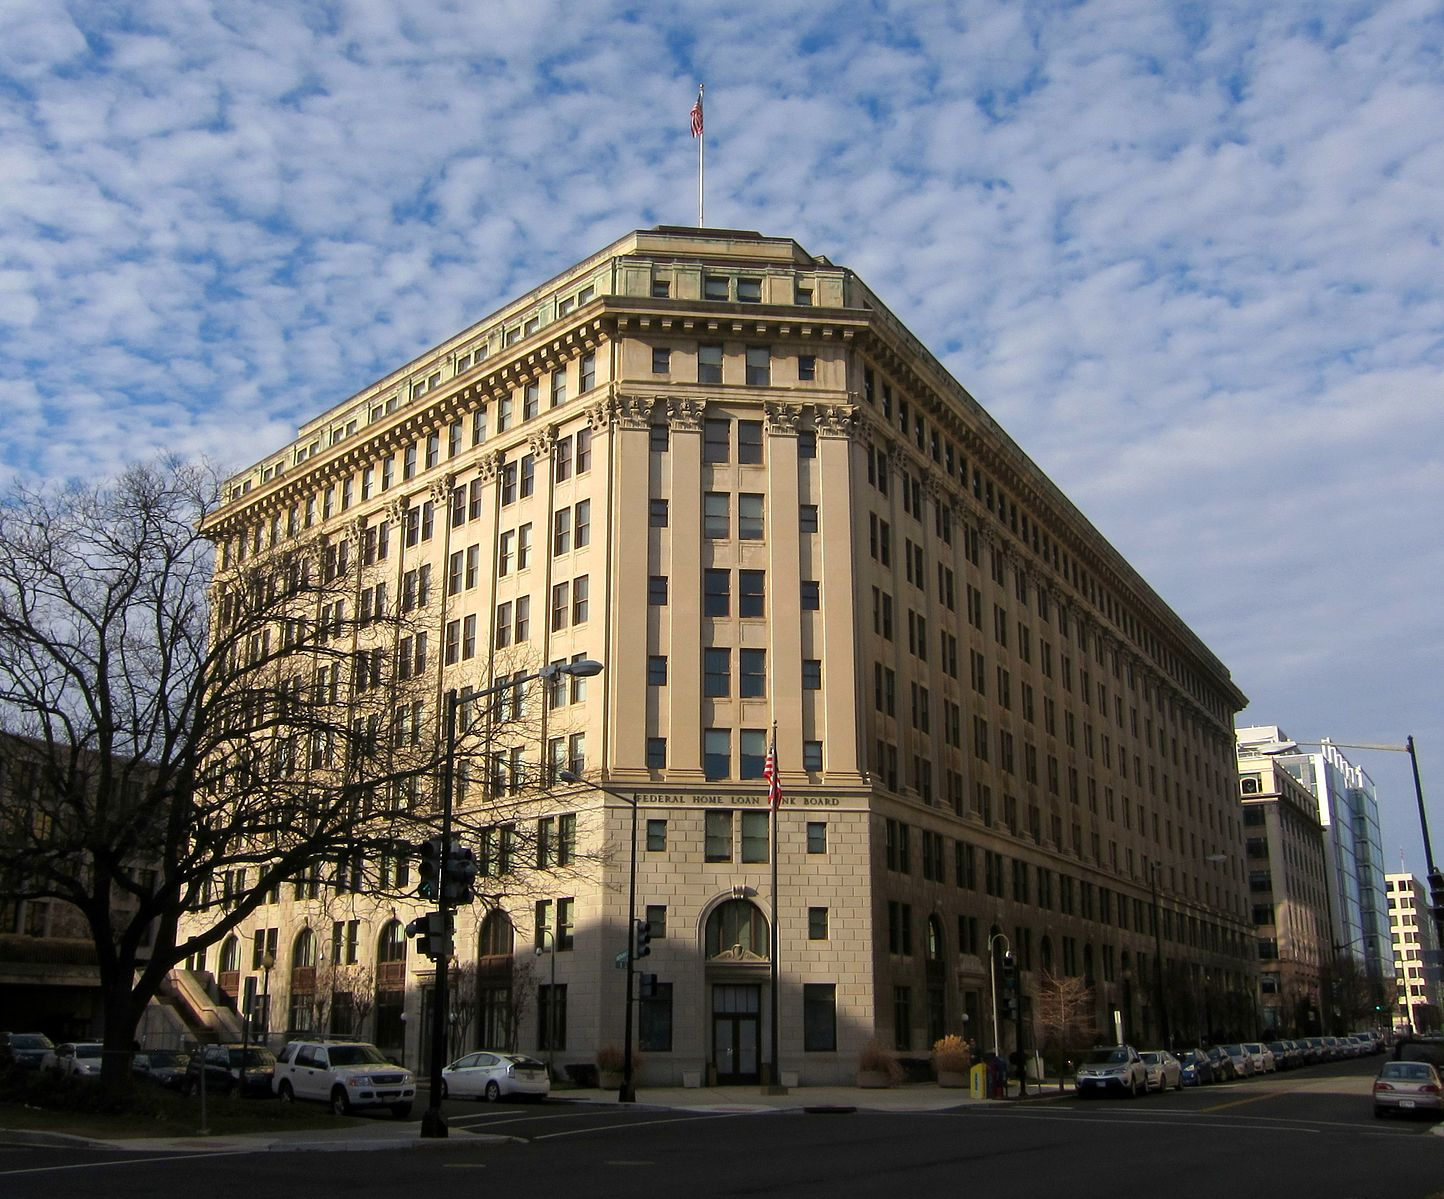
\includegraphics[width = .7\textwidth]{figures/holc_building}\hfill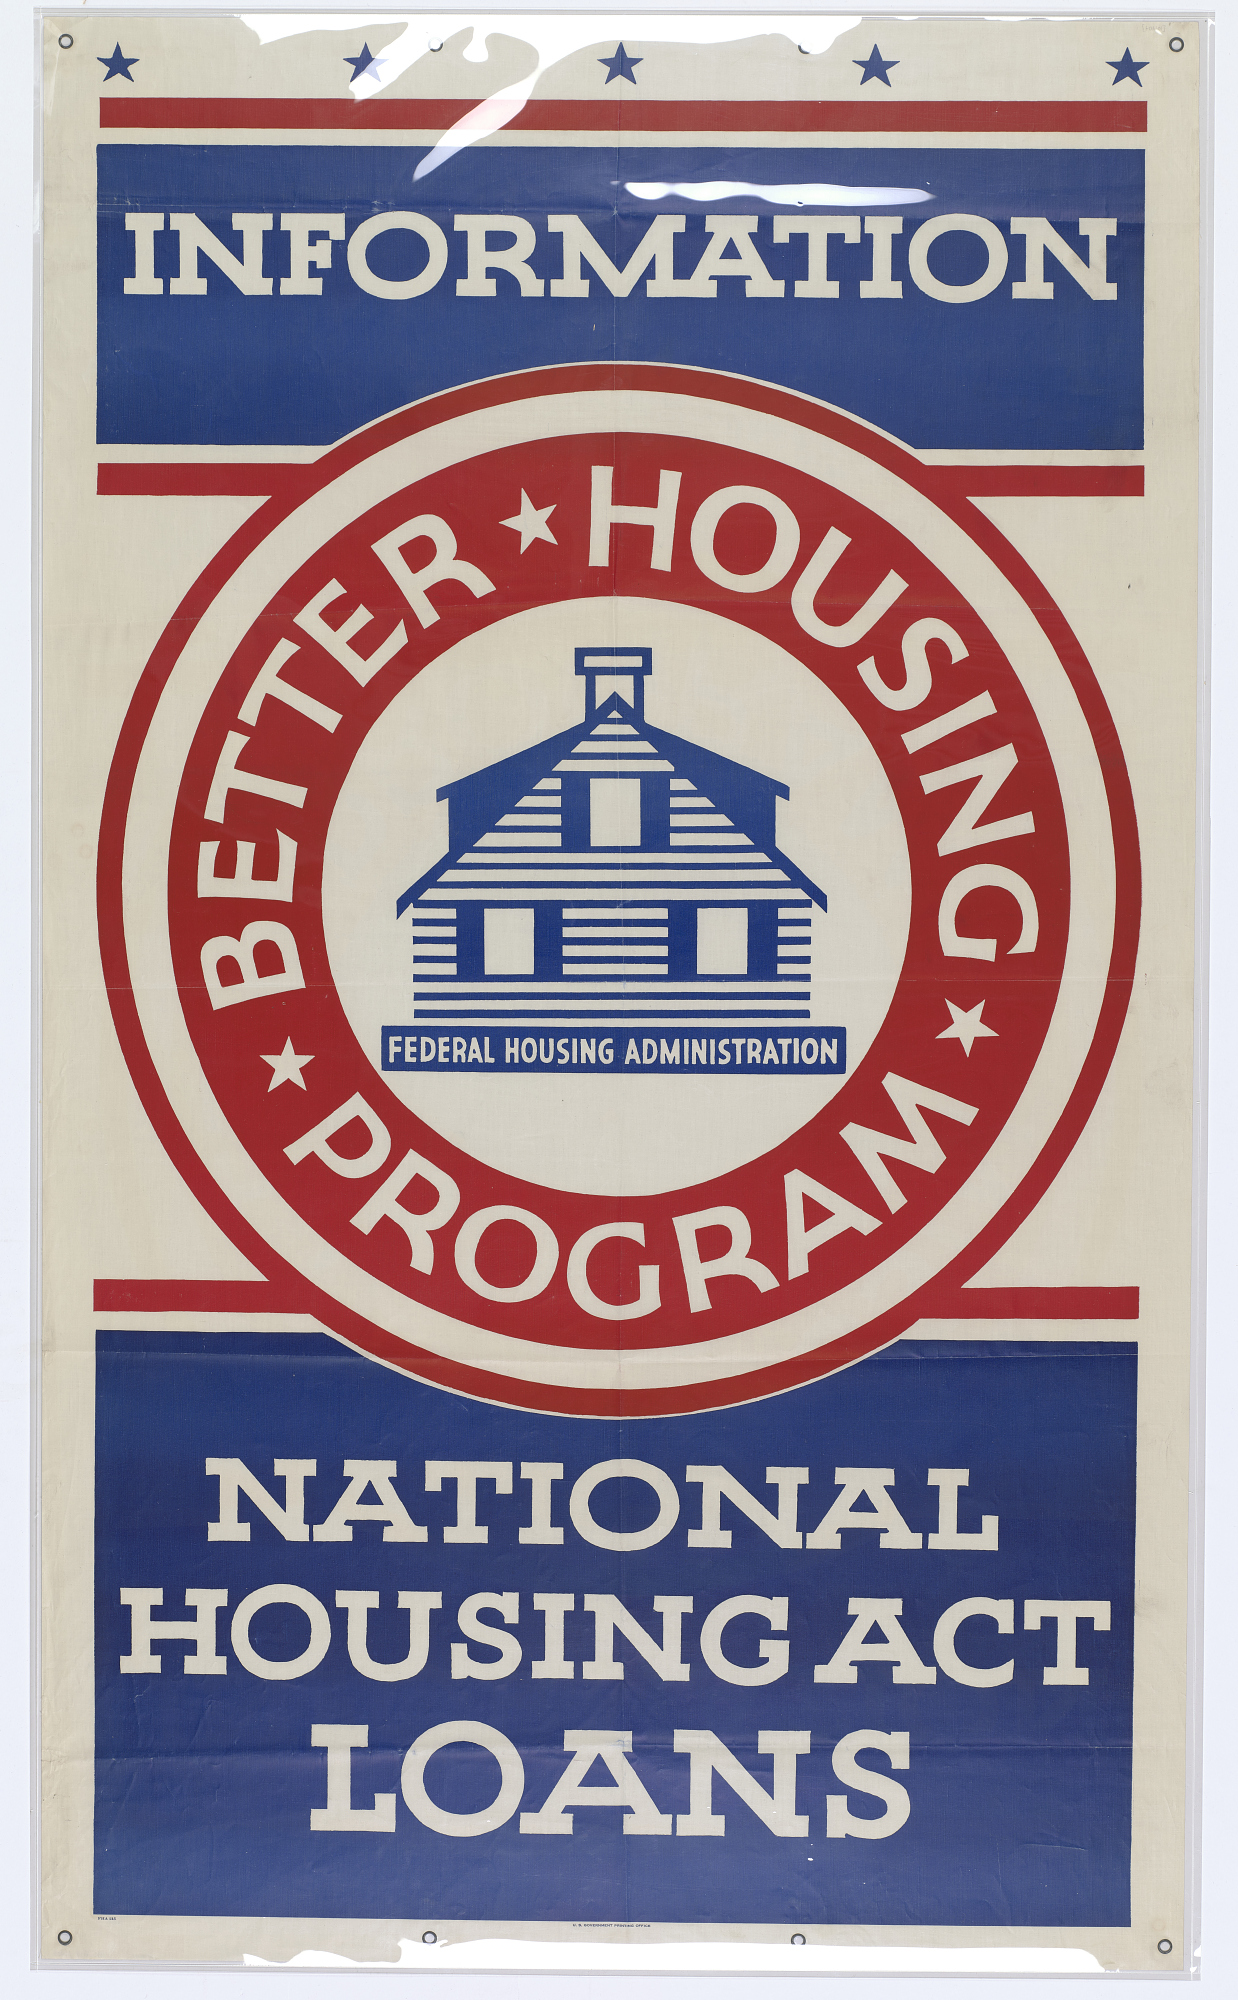
\includegraphics[width = .25\textwidth]{figures/fha_brochure}\\
\begin{footnotesize}
Source: \href{https://commons.wikimedia.org/wiki/File:Federal_Home_Loan_Bank_Board_Building_1.jpg}{Wikimedia} \hfill Source: \href{https://sova.si.edu/details/NMAH.AC.0433\#ref10139}{Smithsonian}
\end{footnotesize}
\end{frame}

\begin{frame}
Home Owners Loan Corporation is tasked with backing mortgages\vskip .2in \pause
They decide to rate neighborhoods
\begin{itemize}
\item \textcolor{seagreen}{A (most desirable)}
\item \textcolor{blue}{B (less desirable)}
\item \textcolor{mustard}{C (declining)} 
\item \textcolor{red}{D (undesirable)}
\end{itemize} \pause \vskip .2in
How? \pause\hfill \bred{(redlining)} \pause
\begin{itemize}
\item Low-income immigrants $\rightarrow$ \textcolor{red}{D grade} \pause
\item Black families $\rightarrow$ \textcolor{red}{D grade}
\end{itemize} \vskip .1in \pause
\begin{footnotesize}
Jackson, Kenneth T. \bref{https://books.google.com/books?hl=en&lr=&id=pqRoAgAAQBAJ}{Crabgrass frontier: The suburbanization of the United States.} Oxford University Press, 1987.
\end{footnotesize}
\end{frame}

\begin{frame}
\includegraphics<1>[width = \textwidth]{figures/holc-scan-la}
\only<1>{Source: Nelson and Ayers, \bref{https://dsl.richmond.edu/panorama/redlining/}{Mapping Inequality}}
\only<2->{
\includegraphics[width = .48\textwidth]{figures/holc-scan-la} \hfill
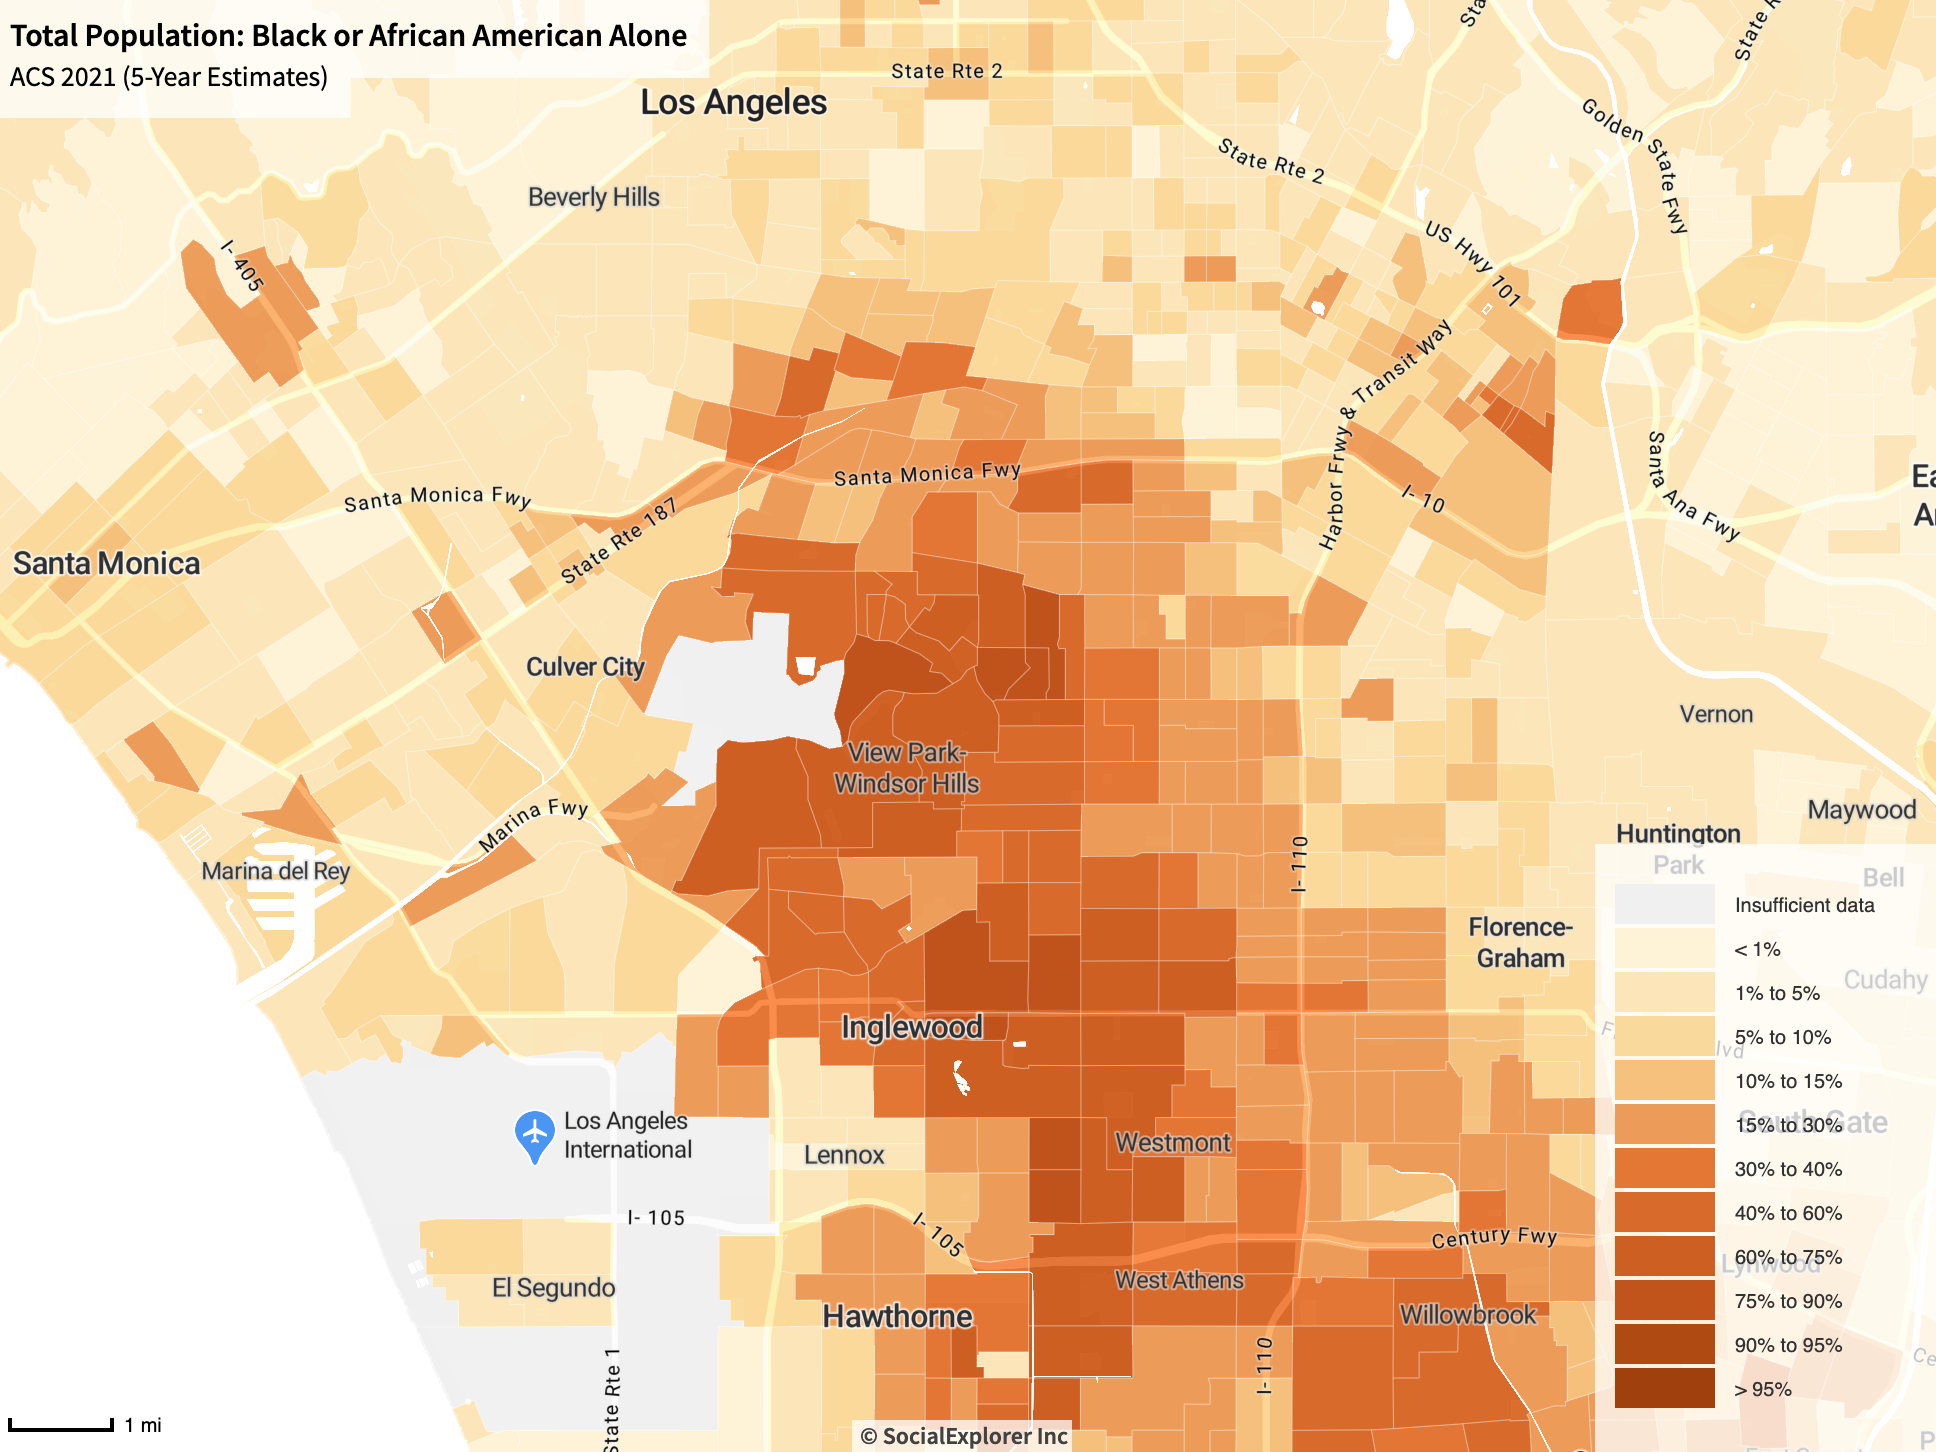
\includegraphics[width = .48\textwidth]{figures/se_la} \\
\begin{footnotesize}
Source: Nelson and Ayers, \hfill Source: \bref{http://resolver.library.cornell.edu/misc/6268440}{Social Explorer}\\ \bref{https://dsl.richmond.edu/panorama/redlining/}{Mapping Inequality}
\end{footnotesize}
}
\end{frame}

\begin{frame}
\includegraphics<1>[height = \textheight]{figures/holc-scan-buffalo}
\only<2->{
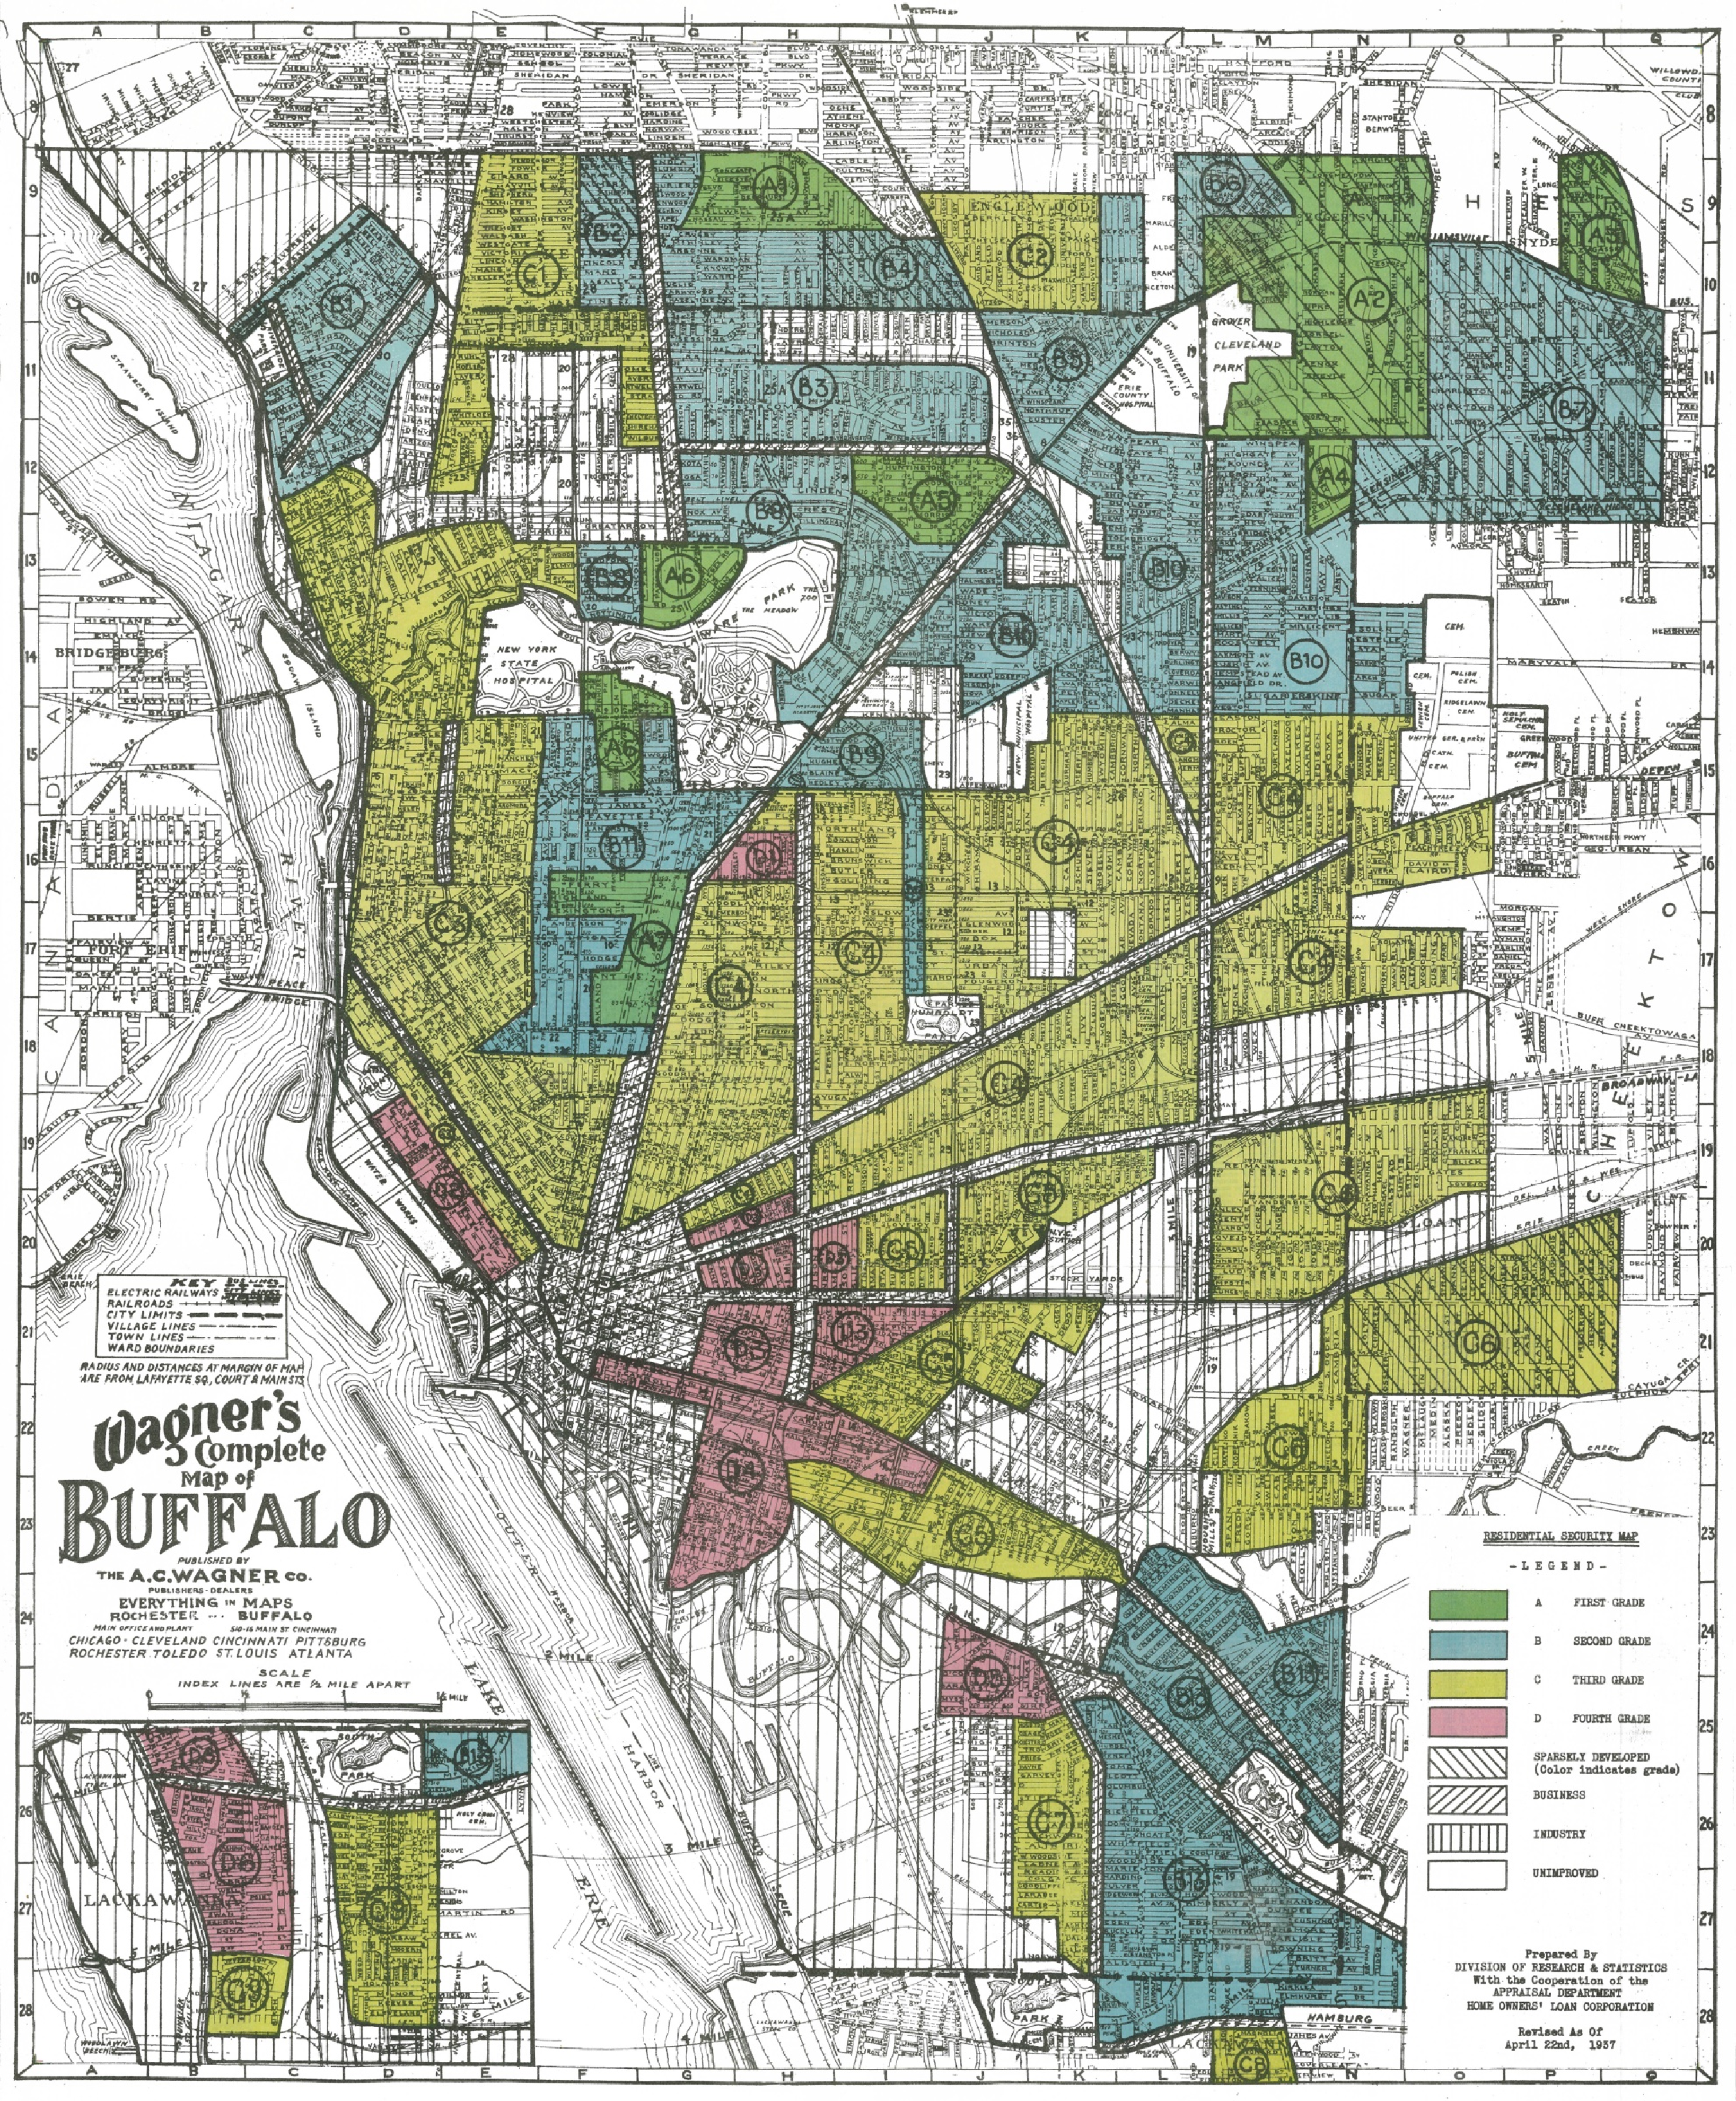
\includegraphics[width = .35\textwidth]{figures/holc-scan-buffalo}\hfill
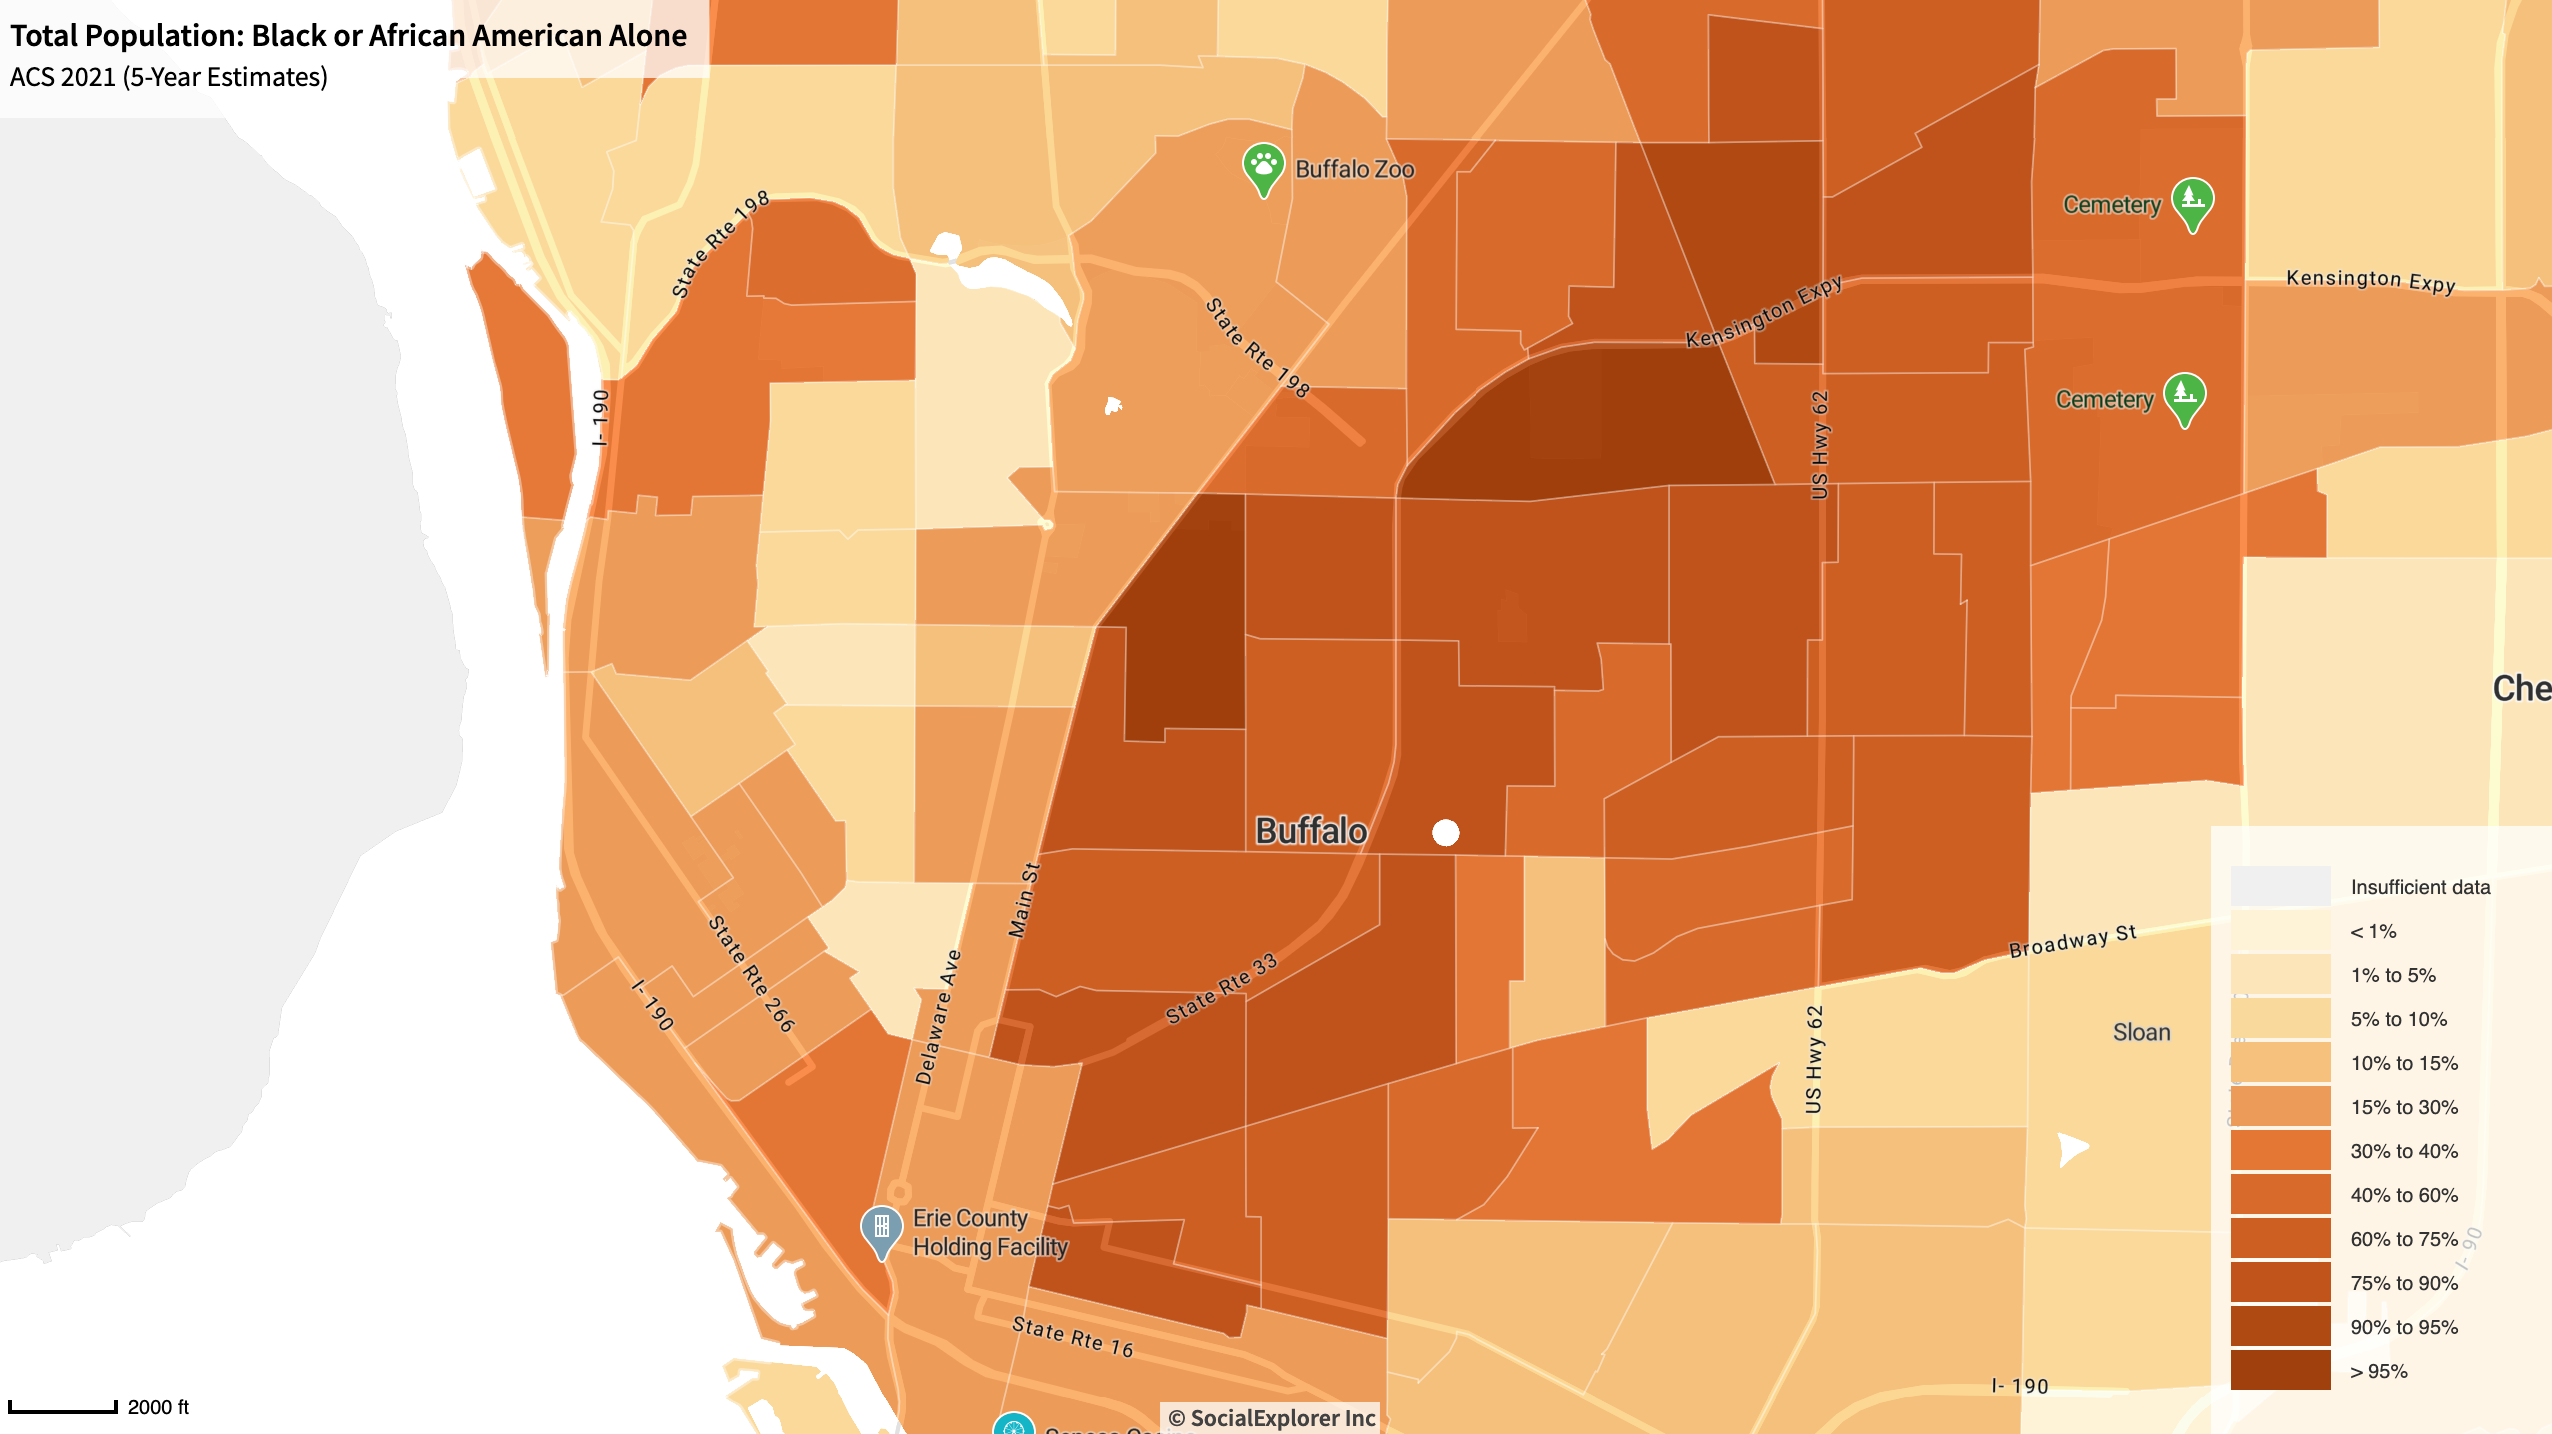
\includegraphics[width = .6\textwidth]{figures/se_buffalo}\\
\begin{footnotesize}
Source: Nelson and Ayers, \hfill Source: \bref{http://resolver.library.cornell.edu/misc/6268440}{Social Explorer}\\ \bref{https://dsl.richmond.edu/panorama/redlining/}{Mapping Inequality}
\end{footnotesize}
}
\end{frame}

\begin{frame}
\includegraphics<1>[height = \textheight]{figures/holc-scan-chicago}
\only<2->{
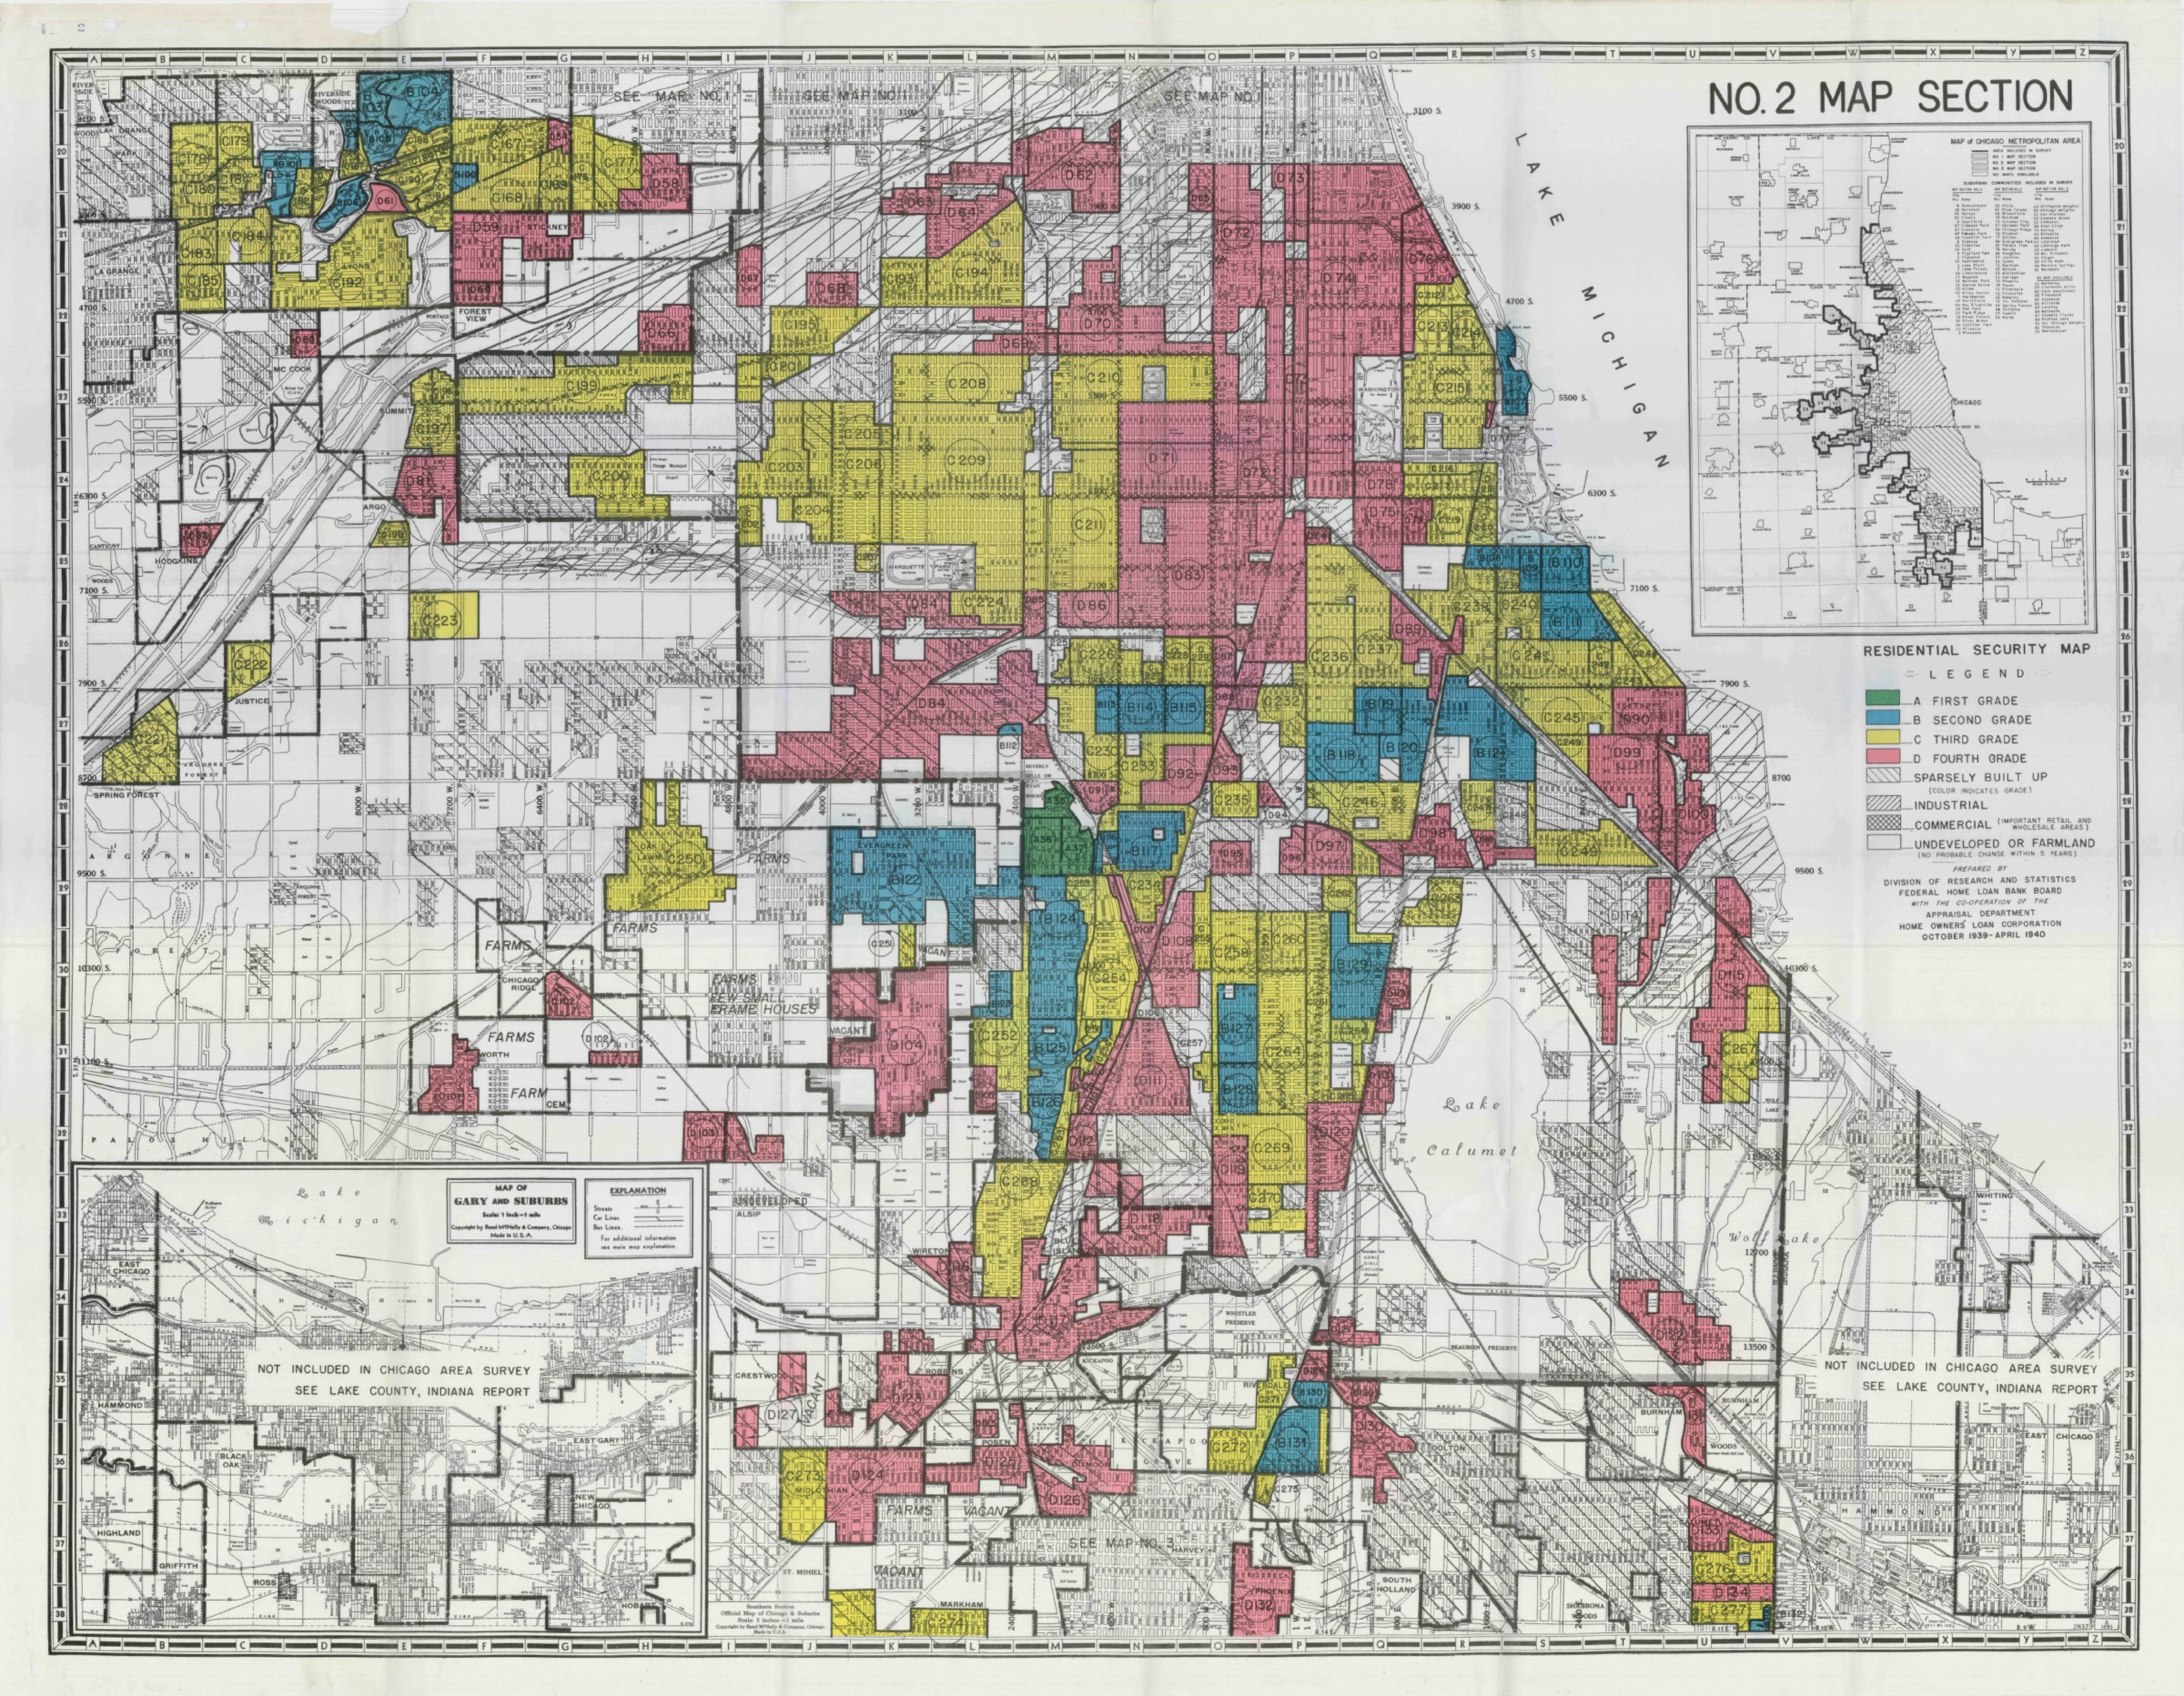
\includegraphics[width = .35\textwidth]{figures/holc-scan-chicago}\hfill
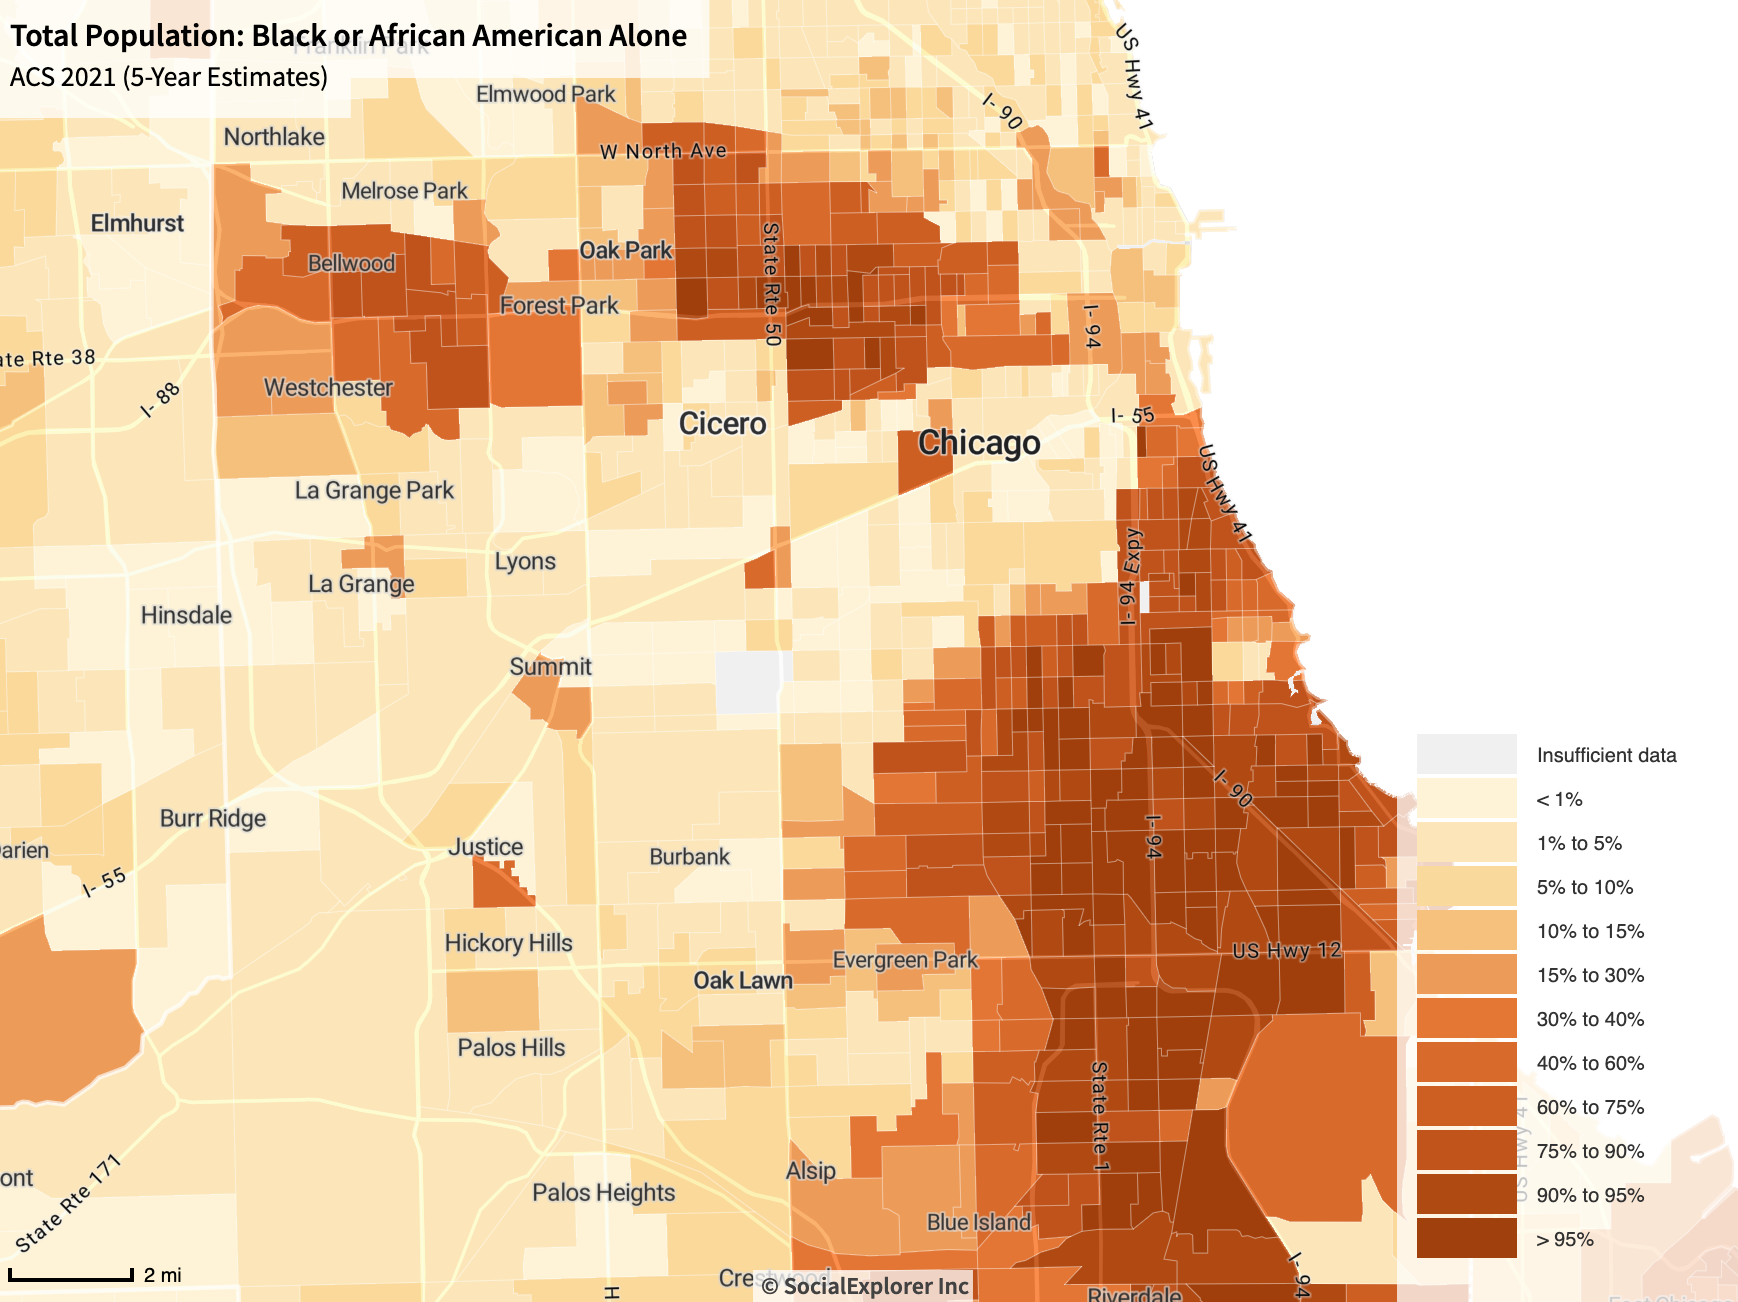
\includegraphics[width = .6\textwidth]{figures/se_chicago}\\
\begin{footnotesize}
Source: Nelson and Ayers, \hfill Source: \bref{http://resolver.library.cornell.edu/misc/6268440}{Social Explorer}\\ \bref{https://dsl.richmond.edu/panorama/redlining/}{Mapping Inequality}
\end{footnotesize}
}
\end{frame}

\begin{frame}{Local organizations furthered racist policies}
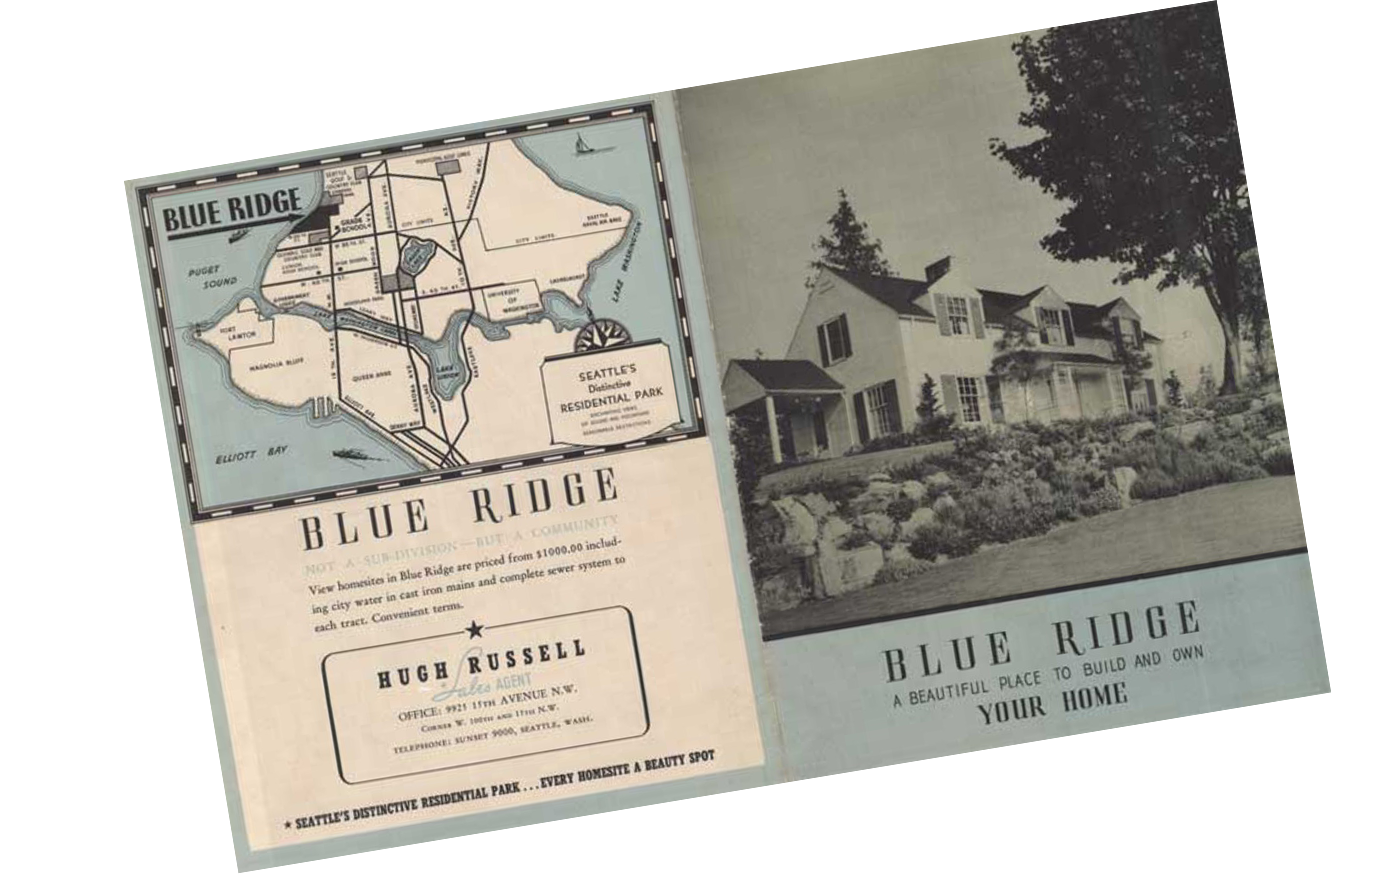
\includegraphics[width = \textwidth]{figures/blueridge_brochure}\\
Source: \href{https://blueridgeseattle.com/about-us/}{Blue Ridge Seattle}
\end{frame}

\begin{frame}{Local organizations furthered racist policies}

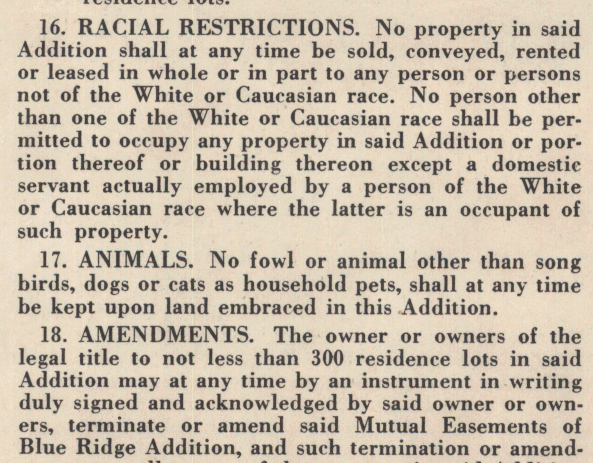
\includegraphics[width = .7\textwidth]{figures/racial_covenant}

\begin{footnotesize}
Source: \href{https://depts.washington.edu/covenants/segregation.shtml}{Civil Rights and Labor History Consortium, University of Washington}
\end{footnotesize}
\end{frame}

\begin{frame}

Explicitly racist policies had lasting consequences

\end{frame}

\begin{frame}

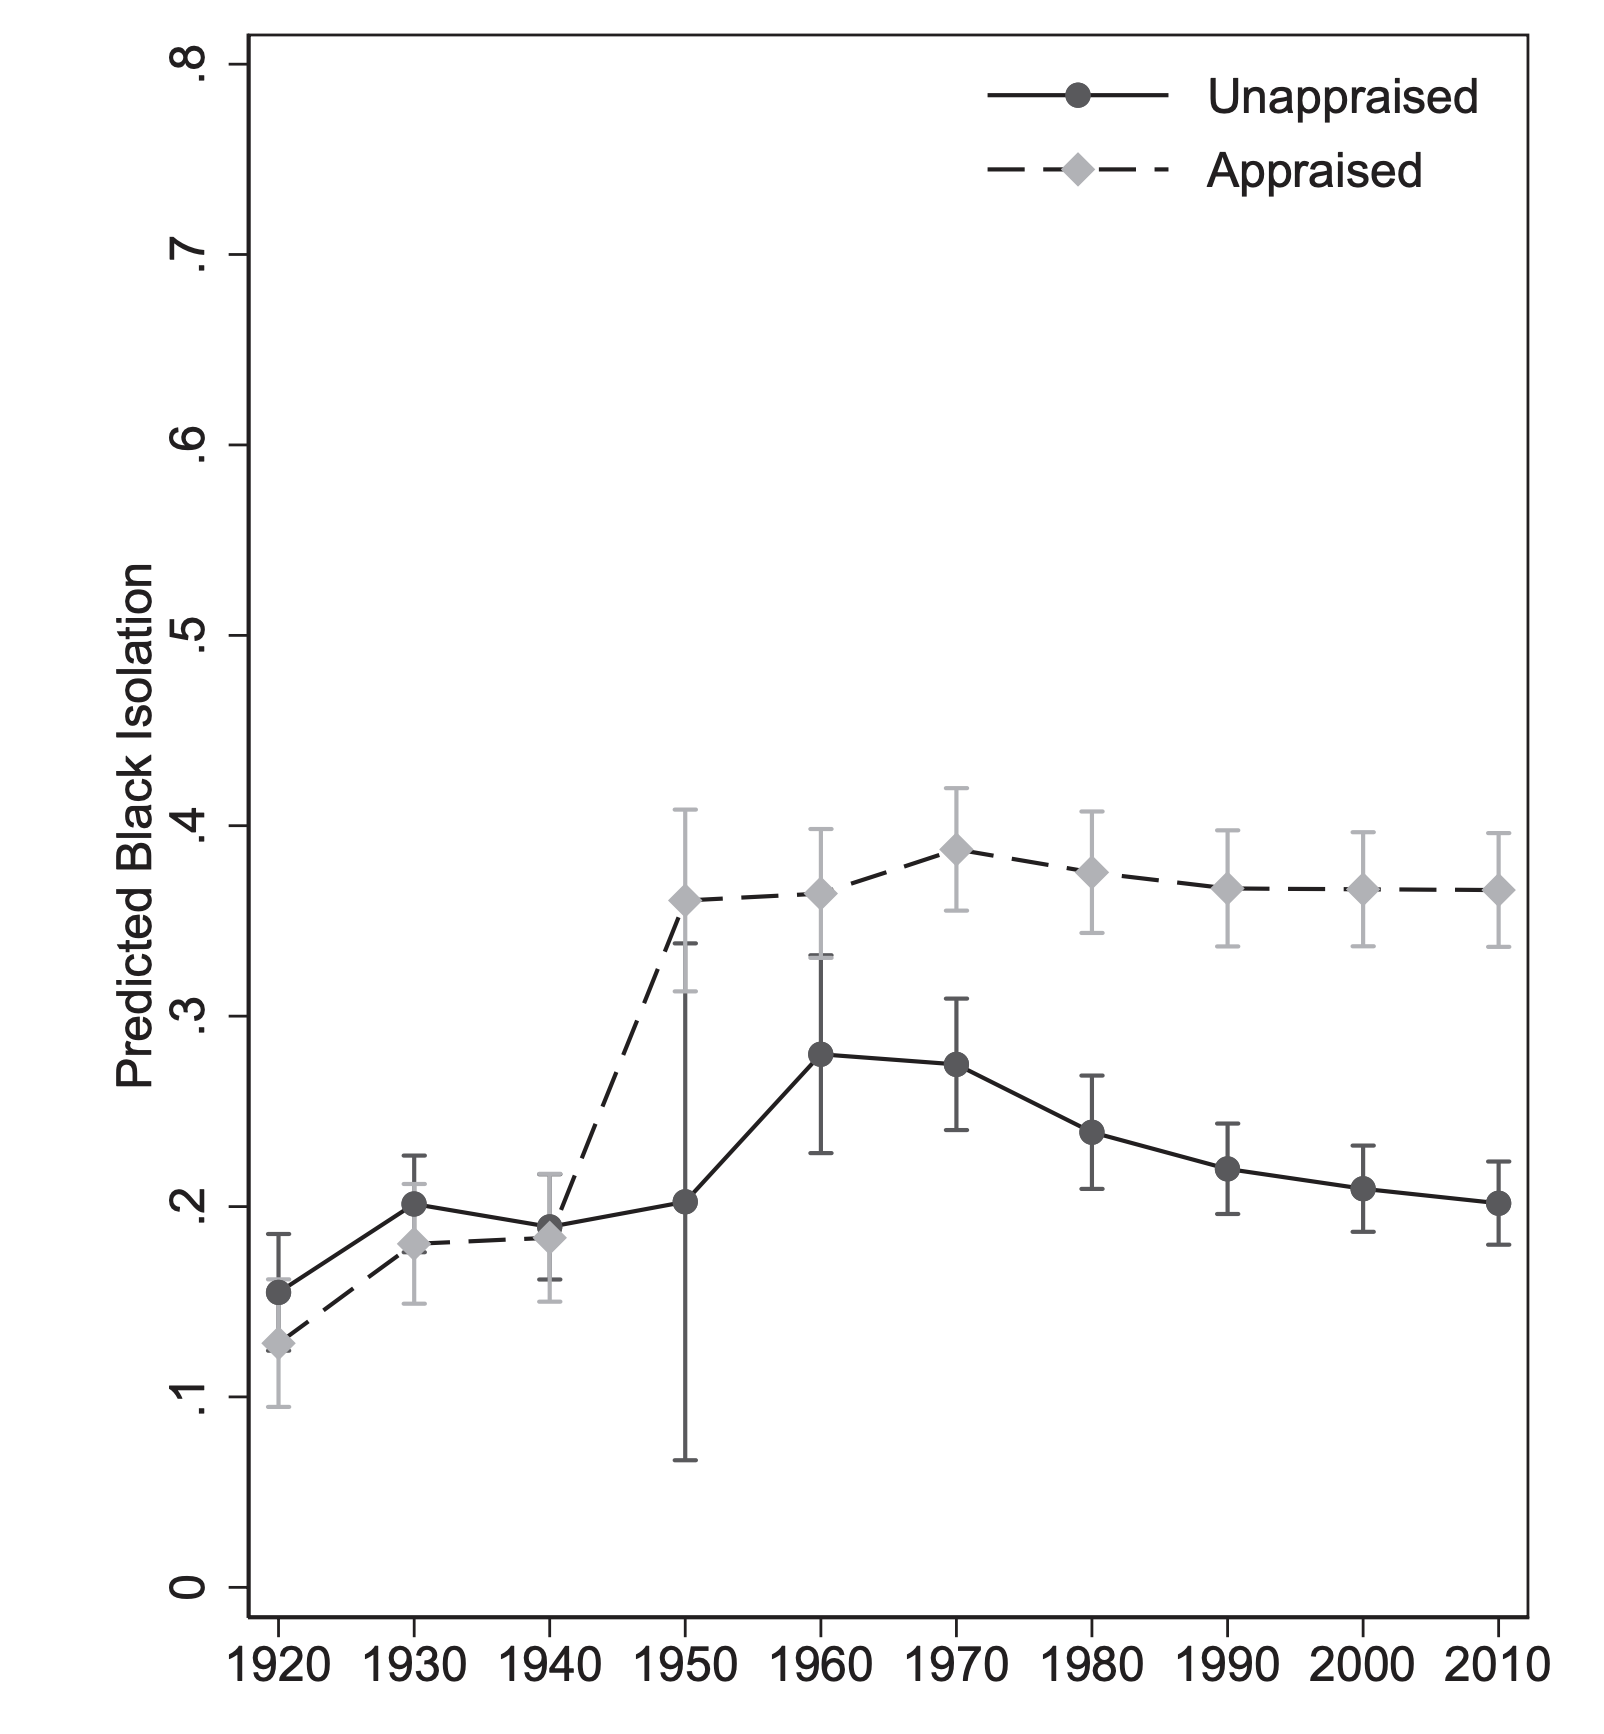
\includegraphics[height = .8\textheight]{figures/faber_fig1}

\begin{footnotesize}
Figure 1 from Faber, J. W. 2020. \bref{https://doi.org/10.1177/0003122420948464}{We built this: Consequences of New Deal era intervention in America’s racial geography.} American Sociological Review, 85(5), 739-775.
\end{footnotesize}
\end{frame}

\begin{frame}{Wealth consequences of redlining} \pause
In redlined neighborhoods, \pause
\begin{itemize}
\item Hard to sell your home \pause
\item Hard to buy a home \pause
\item Home prices do not rise \pause
\end{itemize} \vskip .2in
In the suburbs, \pause
\begin{itemize}
\item Home ownership skyrockets
\begin{itemize}
\item 44\% owned their home in 1940 \hfill National estimates
\item 62\% in 1960 \hfill from \href{https://www.census.gov/data/tables/time-series/dec/coh-owner.html}{U.S. Census}
\end{itemize} \pause
\item Home prices rise \pause
\item Wealth grows
\end{itemize} \vskip .2in \pause
Oliver, M., \& Shapiro, T. (2013). \bref{https://www.taylorfrancis.com/books/mono/10.4324/9780203707425/black-wealth-white-wealth-melvin-oliver-thomas-shapiro}{Black wealth/white wealth: A new perspective on racial inequality.} Routledge.
\end{frame}

\begin{frame}{Additional resources}
\footnotesize
\begin{itemize}
\item Oliver, M., \& Shapiro, T. 2013. \bref{https://www.taylorfrancis.com/books/mono/10.4324/9780203707425/black-wealth-white-wealth-melvin-oliver-thomas-shapiro}{Black wealth / white wealth: A new perspective on racial inequality.} Routledge.
\item Faber, J. W. 2020. \bref{https://doi.org/10.1177/0003122420948464}{We built this: Consequences of New Deal era intervention in America’s racial geography.} American Sociological Review, 85(5), 739-775.
\item Massey, D. S., \& Denton, N. A. 1993. \bref{https://www.hup.harvard.edu/catalog.php?isbn=9780674018211}{American apartheid: Segregation and the making of the underclass.} Harvard University Press.
\item Killewald, A., Pfeffer, F. T., \& Schachner, J. N. 2017. \bref{https://doi.org/10.1146/annurev-soc-060116-053331}{Wealth inequality and accumulation.} Annual Review of Sociology, 43, 379.
\end{itemize}
\end{frame}

\begin{frame}{What will we do next?}

Over the next few classes,
\begin{enumerate}
\item Map racial segregation using \bref{http://resolver.library.cornell.edu/misc/6268440}{Social Explorer}
\item Document \bref{https://info3370.github.io/lessonplans/6b/}{racial wealth gaps} by coding in R
\item Discuss normatively should be done
\end{enumerate}

\end{frame}

\end{document}

